\chapter{基于单张非受限环境照片的人脸重建实现}
\label{chap:recon}

本章介绍了一种非常通用的人脸重建任务的实现,它能够从单张非受限环境照片中重建人脸的3D模型。
非受限环境照片指的是在室外或室内的自然光照条件下,使用手机等非专业设备拍摄的照片。
这类照片的中背景和环境光照通常都比较复杂,且受限于拍摄条件难以显式建模或捕获。
该实现输出的模型可用于人脸编辑、人脸表情迁移、语音驱动等下游任务,
并支持在小范围视角和光照变化下重新渲染,输出较高质量的图像。

现有方法或者使用多帧、多视角监督,或者借助分割结果或人脸2D关键点检测结果辅助监督。
这些方法或对数据要求高,或有较严重的传递误差,或需要额外的人工标注。
本文则只使用单张照片,通过第\ref{chap:method}章中提出的方法,主要利用可微分渲染中可见性梯度提供的监督信号完成重建。
与使用2D关键点监督的方法相比,本文的方法无需除照片外的监督信息,并能利用照片中的每一个像素,实现更加稠密的监督,从而理论上提升重建的精度。

本章的主要内容包括:
在应用第\ref{chap:method}章中提出的方法计算人脸模型的可见性梯度时,人脸模型裁剪时产生的人为制造的边缘在照片中并无对应,会产生错误的梯度,引导模型过度扩张。
本章提出了一种使用SDF贴图的方法以排除这些梯度的干扰。
此外,为了提升逆渲染优化的鲁棒性,本章集成现有神经网络和3DMM人脸模型以提供正则化;
为了重现高分辨率的输入图像中的更多细节,本章还使用了一些传统算法以生成高分辨率的纹理贴图。

\section{总体流程}

\begin{figure}
\centering
\begin{tikzpicture}[
    node distance=1cm and 1.2cm,
    data/.style={draw, ellipse, minimum size=1cm, align=center},
    proc/.style={draw, rectangle, minimum size=1cm, align=center},
    every edge/.style={draw, ->},
]
    \zihao{5}
    \node[data] (img) {照片};
    \node[proc, right=of img] (net) {神经网络};
    \node[proc, right=of net] (inv) {逆渲染};
    \node[proc, right=of inv] (trans) {纹理迁移};
    \node[proc, right=of trans] (decom) {光照解耦};
    \node[proc, right=of decom] (comp) {纹理补全};
    \node[data, above left=of inv] (3dmm) {3DMM};
    \node[data, below=of inv] (light) {环境光照};
    \node[data, above right=of inv] (tex) {低频纹理};

    \path (img) edge (net)
          (net) edge node [above] {初始化} (inv)
          (inv) edge node [above] {几何} (trans)
                edge (light)
                edge (tex)
          (trans) edge node [above] {贴图} (decom)
          (decom) edge node [above] {贴图} (comp)
          (3dmm) edge (inv);
    \path[every edge] (light) -| (decom);
    \path[every edge] (tex) -| (comp);
\end{tikzpicture}
\caption{人脸重建总体流程}
\label{fig:recon_overall}
\end{figure}
为完成该人脸重建的目标,本方法将输出一个基于预定义的拓扑结构的三角形网格,以及其对应的高清纹理贴图,该图的像素中编码了人脸表面的光线反射率。
其总体流程如\ref{fig:recon_overall}所示。
本文首先利用现有方法\citep{deep3d}根据输入的照片估计3DMM人脸模型的形变系数,环境光照,人脸姿态等信息。
以此作为初始化,本文利用第\ref{chap:method}章提出的方法进一步将模型精确对齐到输入照片中,并进一步优化对环境光照和人脸姿态的估计。
然后本文将照片的像素投影到纹理空间,依据估计的环境光照将照片中的光照效果和人脸本身的反射率分离,以支持渲染时的光照变化。
最后,本文利用3DMM建模的低频纹理对模型在照片中被遮挡的部分进行补全,以支持渲染时视角的变化。

后文将对该流程中的每个步骤进行详细介绍。

\section{基于神经网络回归的模型初始化}
\label{sec:recon_init}

基于可微分渲染的逆渲染方法通常难以处理较大的姿态变化,它容易在复杂的非线性优化中陷入局部最优。
因而之前很多方法均使用了2D人脸关键点检测结果以提供大范围的,较为平滑的监督信号。
然而关键的的位置定义是较为模糊的,3D模型上的标注误差和2D检测的误差都会传递到之后的步骤中。
而本文则不使用关键点以避免这些传递误差,同时免去模棱两可的3D模型关键点标注工作。
本文提出利用现有神经网络方法\citep{deep3d}通过输入照片估计其中人脸3DMM模型的形变系数,环境光照,人脸姿态等信息,并以此作为下一步骤的初始化。

\paragraph{人脸检测}
具体来说,对于一张输入的照片$\mathcal{I}\in\mathbb{R}^{H\times W\times 3}$,本文首先在其中检测人脸。
在输入前本文首先对照片$\mathcal{I}$进行$N$倍降采样(平均池化)为$\mathcal{I}_m$以控制检测的资源消耗,其中$N=\left\lceil \max(H, W) / 1024\right\rceil$,也就是将最长边控制在1024像素以内。
本文使用了\citet{SFD}开源的人脸检测软件。
该软件能输出矩形人脸检测框,本文选择其输出的面积最大的检测框$B$。

\paragraph{系数预测}
然后本文进一步将照片$\mathcal{I}_m$裁剪并降采样为$\mathcal{I}_s\in\mathbb{R}^{224\times 224\times 3}$,将检测框包含在其中并使其面积最大且居中。
若裁剪框超出像素边缘则填充黑色,以保持人脸在图像中心。
然后$\mathcal{I}_s$将输入到\citet{deep3d}开源的软件中,
它将输出BFM模型\citep{BFM}的
人脸身份系数$\mathbf{\alpha}_\mathrm{id}\in\mathbb{R}^{80}$,
人脸表情系数$\mathbf{\alpha}_\mathrm{exp}\in\mathbb{R}^{64}$,
人脸纹理系数$\mathbf{\alpha}_\mathrm{tex}\in\mathbb{R}^{80}$,
人脸姿态$\mathbf{M}_\mathrm{d}\in\mathrm{SE(3)}$,
环境球谐光照系数$\mathbf{\gamma}\in\mathbb{R}^{9\times 3}$。
其中涉及到的相机坐标系的3D坐标均可通过约定的投影矩阵$\mathbf{P}_\mathrm{d}$投影回图像平面,并与输入图像$\mathcal{I}_s$较好地对齐。

\paragraph{坐标系转换}
然而,上一步骤预测时使用的投影矩阵是固定的,而输入的照片拍摄时使用的设备,人脸在照片中的尺寸,位置都有不同。
为了获取尽可能精确的结果,本文试图从照片的元数据中提取相机实际参数,结合裁减的方式,计算更准确的投影矩阵,并将所涉及到的3D坐标在不同投影矩阵间进行转换,同时满足:3D点在图像上投影的位置基本不变;人脸模型在3D空间的尺度基本不变。

此处投影矩阵定义为$3\times 3$的矩阵$\mathbf{P}$,其使用方式为$\mathbf{x} = \mathbf{P}\mathbf{X}$,
其中$\mathbf{X}$为相机坐标系下的点的三维坐标,$(\mathbf{x}_x/\mathbf{x}_z,\mathbf{x}_y/\mathbf{x}_z)\in[-1,1]^2$即是该点投影到图像上的二维坐标。
注意此处的图像坐标系与图像分辨率无关,这与OpenGL等渲染库的约定一致,且便于后续在不同投影矩阵转换时的计算。
但与OpenGL中常用的投影矩阵形式不同,为了简化推导,此处的投影矩阵并未投影深度。
可从照片的EXIF中提取的信息包括相机焦距$f\in\mathbb{R}$,分辨率$\mathbf{r}\in\mathbb{R}^2$,传感器像素密度$\mathbf{\rho}\in\mathbb{R}^2$。
根据这些信息,并假设该相机符合完美的小孔成像模型,则该相机的投影矩阵为:
\begin{equation}
    \mathbf{P}_\mathrm{cam} = \begin{bmatrix}
        \frac{2f\mathbf{\rho}_x}{\mathbf{r}_x} & 0 & 0 \\
        0 & \frac{2f\mathbf{\rho}_y}{\mathbf{r}_x} & 0 \\
        0 & 0 & 1
    \end{bmatrix}
    \text{。}
\end{equation}
进一步地,裁减操作可以看作是平移和缩放操作的组合,记裁剪框的左下角和右上角坐标分别为$\mathbf{p}_\mathrm{min},\mathbf{p}_\mathrm{max}\in[-1,1]^2$,
则裁剪框内区域的投影矩阵为:
\begin{equation}
    \mathbf{P}_\mathrm{crop} = \begin{bmatrix}
        \frac{2}{\mathbf{p}_\mathrm{max,x}-\mathbf{p}_\mathrm{min,x}} & 0 & 0 \\
        0 & \frac{2}{\mathbf{p}_\mathrm{max,y}-\mathbf{p}_\mathrm{min,y}} & 0 \\
        0 & 0 & 1
    \end{bmatrix}\begin{bmatrix}
        1 & 0 & -\frac{\mathbf{p}_\mathrm{min,x}+\mathbf{p}_\mathrm{max,x}}{2} \\
        0 & 1 & -\frac{\mathbf{p}_\mathrm{min,y}+\mathbf{p}_\mathrm{max,y}}{2} \\
        0 & 0 & 1
    \end{bmatrix}\mathbf{P}_\mathrm{cam}
    \text{。}
\end{equation}

以下将介绍具体如何将3D模型从投影矩阵$\mathbf{P}_\mathrm{d}$转换到$\mathbf{P}_\mathrm{crop}$下。
该转换分为两步,将模型关于相机旋转以保持模型中心点投影位置不变,再将模型向朝向或远离相机的方向平移以保持模型的投影尺度不变。
这两步操作均为刚性变换,因此可以保证模型在3D空间的尺度不变。

首先求解旋转,该步骤主要用于平衡不同照片中人脸裁剪框位置的差异。
记3D网格模型$M=\{\mathbf{v}_i\}_i$为三维顶点的集合,其中$\mathbf{v}_i\in\mathbb{R}^3$为神经网络预测的顶点的三维坐标。
记$\bar{\mathbf{v}} = \frac{1}{|M|}\sum_{i=1}^{|M|}\mathbf{v}_i$为模型中心点的三维坐标。
若要该中心点的投影位置不变,则该点应位于新坐标系下的一条以原点为起点的射线上,该射线上另一点的坐标为$\bar{\mathbf{v}}' = \mathbf{P}_\mathrm{crop}^{-1}\mathbf{P}_\mathrm{d}\bar{\mathbf{v}}$。
因此,所需旋转的旋转轴为$\bar{\mathbf{v}}' \times \bar{\mathbf{v}}$,
旋转角为$\arccos\left(\frac{\bar{\mathbf{v}}'\cdot\bar{\mathbf{v}}}{\|\bar{\mathbf{v}}'\|\|\bar{\mathbf{v}}\|}\right)$。
可由罗德里格斯公式计算其对应旋转矩阵$\mathbf{R}$。
旋转后的中心点坐标记为$\bar{\mathbf{v}}'' = \mathbf{R}\bar{\mathbf{v}}$。

然后可以求解所需平移,该步骤主要用于平衡不同相机的焦距参数的差异。
记平移后的中心点位置为$\bar{\tilde{\mathbf{v}}} = s\bar{\mathbf{v}}''$,
$s$表示平移前后该点据相机的距离比例。
若要模型投影尺度不变,则$s$应满足如下方程:对于三维坐标$\mathbf{x}=[x,y,z]^\mathsf{T}$
\begin{equation}
    \left.\nabla_{x,y}\left(\frac{\mathbf{P}_\mathrm{crop}\mathbf{x}}{z}\right)\right|_{\mathbf{x}=\bar{\tilde{\mathbf{v}}}} =
    \left.\nabla_{x,y}\left(\frac{\mathbf{P}_\mathrm{d}\mathbf{x}}{z}\right)\right|_{\mathbf{x}=\bar{\mathbf{v}}}
    \text{。}
\end{equation}
该方程是超定方程,但由于这里使用的投影矩阵均是按相同比例处理x和y轴的,因此应当能解出一致的$s$。在实践中可以使用最小二乘法求解。

在得到针对模型中心点的变换参数后,可将其合成一个变换矩阵以应用到整个模型的任意顶点上。
变换矩阵为:
\begin{equation}
    \mathbf{M}_\mathrm{t} = \begin{bmatrix}
        \mathbf{I} & \bar{\tilde{\mathbf{v}}} - \bar{\mathbf{v}}'' \\
        \mathbf{0} & 1
    \end{bmatrix}\mathbf{R}
    \text{,}
\end{equation}
转换后的模型即为$\tilde{M}=\{\mathbf{M}_\mathrm{t}\mathbf{v}_i\}_i$,其中$\mathbf{v}_i$需在最后一维上加上1以扩展为齐次坐标。
% 图\ref{fig:crop}用一个玩具实验展示了转换前后的模型,以及该转换的必要性。

\section{基于SDF贴图的裁剪边缘分类方法}
\label{sec:recon_sdf}

可微分渲染在应用到人脸3D重建时有一个特殊的问题:人是一个很大的物体,而人脸重建的目标通常仅仅是人脸的这一小块区域。
所以通常在人脸重建中用于逆渲染的模型都是裁剪过的,只包含人脸的部分,因此具有一些人为制造的边缘。
这些边缘在照片中并不存在,但第\ref{chap:method}章提出的方法在应用到人脸时却也会在这些边缘产生相关梯度,由于照片中并无对应的边缘可供对齐,这些梯度将导致模型过度扩展,影响最终收敛的效果。

解决该问题的关键在于如何判断渲染图像中的像素与模型指定边缘的位置关系,以便在计算梯度时能够区分人为制造的边缘和真正需要优化的边缘。
在计算机图形学领域,\citet{sdf_glyphs}提出使用SDF(Signed Distance Field,有向距离场)贴图来绘制可任意放大的矢量图形,
并能根据SDF的梯度判断像素在渲染图像中到图形边缘的距离,从而实现各向异性的抗锯齿。
受此启发,本文提出一种简单的基于SDF贴图的方法来区分人为制造的和真正需要优化的边缘。

具体地,本文定义一种SDF贴图。
对于该贴图中的每个像素,其值为一个单通道浮点数$d$,表示在贴图中该像素点到最近的人为制造边缘的距离,在模型内部的为正,模型外部的为负,
如图\ref{fig:sdf}所示。
由于该贴图中并无太多高频信息,本文仅使用了$256 \times 256$的分辨率。
虽然似乎只有模型内部的贴图像素才会在渲染时被采样到,只需要计算模型内部的正值即可,但实际上,由于采样时使用双线性插值,外部的负值也会被采样到从而参与插值计算中。
更准确的线性插值结果正是SDF的主要优势之一。
从图中也可见,无论是SDF值还是其梯度在穿过边缘时都依然是平滑的。

\begin{figure}
\centering
\begin{subfigure}[t]{3.3in}
    \centering
    \import{build/figures/}{sdf.pgf}
    \caption{SDF贴图}
    \label{fig:sdf}
\end{subfigure}
\begin{subfigure}[t]{2.9in}
    \centering
    \import{build/figures/}{sdf_grad.pgf}
    \caption{SDF的梯度}
    \label{fig:sdf_grad}
\end{subfigure}
\caption[SDF贴图可视化]{SDF贴图可视化。灰色线为模型中人为制造的边缘。(a)为SDF贴图,表示每个像素到最近边缘的距离,模型内部为正,外部为负;(b)为(a)的梯度向量,其x和y分量分别可视化为红色和绿色通道。}
\end{figure}

下面以nvdiffrast的工作方式为例说明该贴图的使用方式:
nvdiffrast抗锯齿模块工作时将以一对相邻的像素点为单位(如图\ref{fig:aa}),其中一个像素在模型内部,另一个像素在模型外部。
\def\dgrad{\dot d}
对于处于模型内部的像素,可从SDF贴图中采样其对应的$d$值,并计算其在对应外部像素方向上的梯度$\dgrad$,
也即对3D模型的表面在该内部像素点的位置使用一个平面进行一阶近似,并求外部像素在该近似平面上的位置,以估计外部像素是否在人为制造边缘之外。
正式地,对于一对分别处于模型内外的像素点,其处于人为制造的边缘当且仅当:
\begin{equation}
    d + \max\left(a\cdot \dgrad, \delta\right) < 0
    \text{,}
\end{equation}
此时应该忽略其产生的可见性梯度。其中$\delta=0.1$为人为限制的梯度的最大值,为避免小概率时过大梯度产生过于离谱的结果;$a=1.5$为梯度放大的系数,为避免偶发的由于精度不足导致的检测遗漏。
这两个超参数的选择对最终结果的影响不大。

\begin{figure}
\centering
\begin{tikzpicture}[
    every node/.style={inner sep=0, anchor=south west},
]
    \node (a) at (0,0) {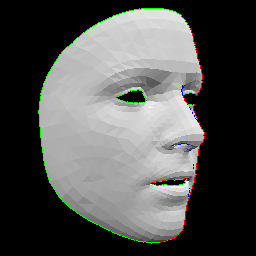
\includegraphics[height=5cm]{figures/debug_sdf}};
    \draw [red,x=5cm/256, y=5cm/256] (70,8) rectangle (192,72);
    \node (b) [
        draw=red,thick,right=of a,inner sep=0.5\pgflinewidth
    ] {
        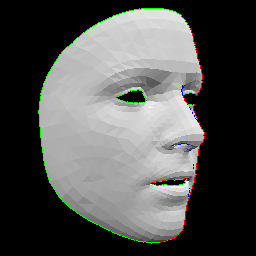
\includegraphics[height=5cm,bb={70 8 192 72},clip]{figures/debug_sdf}
    };
\end{tikzpicture}
\caption[人为制造边缘分类效果]{人为制造边缘分类效果。绿色为人为制造的边缘;红色为与未知背景间的边缘;蓝色为模型内部相互遮挡产生的边缘。}
\label{fig:sdf_result}
\end{figure}

该算法对边缘分类的效果如图\ref{fig:sdf_result}所示。
可见算法将所有边缘分为了三类,
其中绿色为人为制造而需要忽略的边缘,
红色为与未知背景间的边缘,可按照第\ref{chap:method}章提出的方法进行处理,
蓝色为模型内部相互遮挡产生的边缘,应按正常可微分渲染流程处理。
从图中可见一些红色与绿色交错的区域,这是由于这两种边缘本身并没有明确的界限,有时人为制造的边界会正好投影到实际边界附近。
因此本文认为这种现象是十分合理且可接受的。

\paragraph{SDF贴图的计算}
关于SDF的计算方法有很多,下面介绍本文的实现方式。
本文首先使用Blender将3D人脸模型展开至纹理空间,然后在展开后的所有三角形中查找仅属于一个三角形的边做为所谓人为制造的边缘。
并将这些边加入CGAL封装的层次包围盒\footnote{\url{https://doc.cgal.org/latest/AABB_tree/index.html}}数据结构中,以便快速查找。
随后调用OpenGL将所有展开后的三角形光栅化渲染至图像中,得到边缘内部像素的遮罩。
最后,对于贴图中的每个像素,从层次包围盒中查找与其最近的边,计算其与该边的距离$|d|$,并根据遮罩赋予其符号。$d$的梯度方向即为从该像素指向该边上与其最近点的方向(或反方向),模长为$1$。
本方法相比\citet{green2007improved}介绍的穷举方法效率更高,本方法计算$256\times256$分辨率的贴图,使用CPU单线程用时在10毫秒左右。

\paragraph{梯度计算}
梯度$\dgrad$的计算与所使用的渲染方式有关。
例如OpenGL支持通过数值方法直接求任意变量关于像素坐标的梯度\footnote{\url{https://registry.khronos.org/OpenGL-Refpages/gl4/html/dFdx.xhtml}}。
而针对本文使用的nvdiffrast来说,本文首先以解析法随SDF一同计算其关于纹理坐标的梯度$\frac{\partial d}{\partial u}$和$\frac{\partial d}{\partial v}$,并将其与$d$一同保存于贴图中。
然后根据nvdiffrast的插值模块给出的纹理坐标和像素坐标间的雅可比矩阵将其转换到像素坐标:
\begin{equation}
    \begin{bmatrix}
        \frac{\partial d}{\partial x} \\
        \frac{\partial d}{\partial y}
    \end{bmatrix} = \begin{bmatrix}
        \frac{\partial u}{\partial x} & \frac{\partial u}{\partial y} \\
        \frac{\partial v}{\partial x} & \frac{\partial v}{\partial y}
    \end{bmatrix} \begin{bmatrix}
        \frac{\partial d}{\partial u} \\
        \frac{\partial d}{\partial v}
    \end{bmatrix}
\text{。}
\end{equation}
该方法与\citet{sdf_glyphs}中提出的方法相同。
所要求的$\dgrad$根据前景和背景像素的相对位置,是$\frac{\partial d}{\partial x}$或$\frac{\partial d}{\partial y}$或其相反数四者之一。

另一种解决该问题的可能的方案是屏蔽位于模型表面特定区域的像素上的可见性梯度,例如屏蔽特定三角形,屏蔽到边缘距离小于某个阈值的区域,手动指定遮罩等。
相比于这些方法,本方法具有如下优势:
\begin{enumerate}
\item 渲染尺度无关:同样的模型区域在不同尺度下渲染呈现的尺度不同,因此屏蔽区域的选择可能需要随着尺度变化而改变。
而本方法融入了$d$对像素坐标的梯度信息,是模型表面的一阶近似,因此不受尺度的影响。
\item 有向性:即使是同一个像素,在其不同方向上也可能分别靠近不同种类的边缘。
本方法通过考虑$d$的梯度方向,可以区分这些不同的边缘。
\end{enumerate}

\section{基于可微分渲染的逆渲染优化}

\begin{figure}
\centering
\begin{tikzpicture}[
    input/.style={draw, minimum width=2.5cm, minimum height=1cm, align=center, font=\small, ellipse, fill=black!10},
    param/.style={input, fill=blue!20},
    intermediate/.style={input, fill=green!20},
    comp/.style={draw, text width=0.6cm, minimum height=1cm, align=center, fill=blue!10},
    legend/.style={minimum width=0.7cm, minimum height=0.7cm},
    node distance=0.3cm and 0.5cm,
]
    \linespread{1.0}
    \node (sdf) [input] {SDF贴图};
    \node (uv) [input, below=of sdf] {纹理坐标};
    \node (tex) [param, below=of uv] {纹理系数};
    \node (id) [param, below=of tex] {身份系数};
    \node (exp) [param, below=of id] {表情系数};
    \node (pose) [param, below=of exp] {姿态};
    \node (delta) [param, below=of pose] {顶点偏移};

    \node (bfm) [comp, right=of id, minimum height=3.6cm, text width=1cm] {BFM};

    \draw [->] (tex) -- (bfm.west |- tex);
    \draw [->] (id) -- (bfm.west |- id);
    \draw [->] (exp) -- (bfm.west |- exp);

    \node (normal) [intermediate, right=of bfm] {顶点法向};
    \node (v) [intermediate, below=of normal] {顶点坐标};
    \node (t) [intermediate, above=of normal] {顶点颜色};
    \node (idx) [input, below=of v] {顶点索引};

    \draw [->] (v) -- (normal);
    \draw [->] (bfm.east |- v) -- (v);
    \draw [->] (bfm.east |- t) -- (t);

    \coordinate (a) at ($(v.west)!0.5!(bfm.east |- v)$);
    \draw (pose) -| (a);
    \draw (delta) -| (a);

    \node (rast) [comp, right=7mm of $(v.east)!0.5!(idx.east)$, minimum height=2.5cm] {光栅化};

    \draw [->] (v) -- node [above, font=\footnotesize] {投影} (rast.west |- v);
    \draw [->] (idx) -- (rast.west |- idx);

    \node (interpolate) [comp, right=of {$(t)!.5!(normal)$} -| rast.east, minimum height=4.9cm] {插值};

    \draw [->] (rast.east |- v) -- (interpolate.west |- v);
    \draw [->] (t)      -- (interpolate.west |- t);
    \draw [->] (normal) -- (interpolate.west |- normal);
    \draw [->] (uv)     -- (interpolate.west |- uv);

    \node (shade) [comp, right=of interpolate.south east, anchor=south west, minimum height=3.6cm] {着色};
    \node (sample) at (shade |- sdf.north) [comp, anchor=north] {纹理采样};
    \node (light) [param, below=0.5cm of shade] {光照系数};

    \draw [->] (light) -- (shade);
    \draw [->] (interpolate.east |- v) -- (shade.west |- v);
    \draw [->] (interpolate.east |- normal) -- (shade.west |- normal);
    \draw [->] (interpolate.east |- t) -- (sample.west |- t);
    \draw [->] (interpolate.east |- uv) -- (sample.west |- uv);
    \draw [->] (sdf) -- (sample.west |- sdf);

    \node (aa) [comp, right=of sample.north east, anchor=north west, minimum height=6.24cm] {抗锯齿};

    \draw [->] (sample) -- (aa.west |- sample);
    \draw [->] (shade) -- (aa.west |- shade);

    \node (out) [intermediate, right=of aa, minimum width=1.6cm] {渲染\\图像};
    \node (photo) [input, below=2.5cm of out, minimum width=1.6cm] {照片};

    \draw [->] (aa) -- (out);
    \draw [->] (photo) -| (aa);
    \draw [<->] (out) -- node [right, font=\small, text width=0.6cm, align=left] {损失函数} (photo);

    \node (l) [anchor=east] at (out.east |- delta) {中间结果};
    \node (l) [left=1mm of l, intermediate, legend] {};
    \node (l) [left=of l] {离散输入};
    \node (l) [left=1mm of l, input, legend] {};
    \node (l) [left=of l] {优化参数};
    \node (l) [left=1mm of l, param, legend] {};

\end{tikzpicture}
\caption{渲染的整体流程}
\label{fig:recon_render}
\end{figure}

基于第\ref{sec:recon_init}节计算的3D模型、纹理、环境光照估计作为逆渲染中渲染参数的初始化,
以及第\ref{chap:method}章和第\ref{sec:recon_sdf}节提出的方法,
本节具体将介绍如何将它们结合nvdiffrast\citep{nvdiffrast}实际应用于人脸3D模型的逆渲染过程中。
渲染的整体流程如图\ref{fig:recon_render}所示。
逆渲染的目标即是通过梯度下降优化的方式,优化模型参数,使得渲染结果与照片尽可能接近。
以下将具体介绍该流程中的各个步骤。

\paragraph{顶点计算和投影}
首先本文实现了类似传统渲染引擎中的顶点着色器的计算。
这个步骤输入模型的各种数据和参数,输出该模型每个顶点在裁切空间中的坐标,以及定义在每个顶点上的一些附加属性。
本文使用的着色模型较为简单,因此附加属性仅包括法线,反射率和纹理坐标。

首先,本文依据类似3DMM模型的方式计算其每个顶点的位置和反射率:
\begin{align}
\mathbf{S} &= \bar{\mathbf{S}} +
\mathbf{B}_\mathrm{id}\mathbf{\alpha}_\mathrm{id} +
\mathbf{B}_\mathrm{exp}\mathbf{\alpha}_\mathrm{exp} +
\mathbf{S}_\mathrm{off}\\
\mathbf{T} &= \bar{\mathbf{T}} +
\mathbf{B}_\mathrm{tex}\mathbf{\alpha}_\mathrm{tex}
\text{。}
\end{align}
其中$\bar{\mathbf{S}}$和$\bar{\mathbf{T}}$分别是平均的人脸形状和反射率,
$\mathbf{B}_\mathrm{id}$、$\mathbf{B}_\mathrm{exp}$和$\mathbf{B}_\mathrm{tex}$分别是身份、表情和反射率的PCA基,并预先根据其对应的标准差进行了放大。
与之前方法\citep{deep3d,GuoZCJZ19}保持一致,本文使用了BFM 2009模型\citep{BFM}中的身份和反射率基,以及从Face Warehouse\citep{FaceWarehouse}中创建的表情基。
$\mathbf{\alpha}_\mathrm{id}$、$\mathbf{\alpha}_\mathrm{exp}$和$\mathbf{\alpha}_\mathrm{tex}$分别是身份、表情和纹理的系数,是所需优化的参数。
与之前的方法不同,本文使用了\ref{sec:recon_init}节中预测的系数来计算$\bar{\mathbf{S}}$和$\bar{\mathbf{T}}$,从而利用神经网络中的知识作为逆渲染优化的先验。
此外,本文还额外对顶点位置增加了一个偏移量$\mathbf{S}_\mathrm{off}$,以允许其偏离PCA产生的低维空间,拟合更加多样的人脸形状,从而充分发挥逆渲染用于监督的信息量大的优势。

在获得顶点位置后,还需将其变换到相机坐标系并投影到裁切空间中,以便后续的光栅化。投影后顶点在裁切空间中的坐标为:
\begin{equation}
\mathbf{S}_\mathrm{clip} = \mathbf{P}_\mathrm{crop}\mathbf{M}_\mathrm{t}\mathbf{M}_\mathrm{d}\mathbf{M}_\mathrm{c}\mathbf{S}
\text{,}
\end{equation}
其中$\mathbf{M}_\mathrm{c}\in \mathrm{SE(3)}$是可优化的参数。
该步骤在之前第\ref{sec:recon_init}节神经网络预测($\mathbf{M}_\mathrm{d}$)和坐标系转换($\mathbf{M}_\mathrm{t}$)后的结果的基础上,再增加了一个参数以给逆渲染进一步优化的空间。
需注意,此处的投影矩阵$\mathbf{P}_\mathrm{crop}$需要选取合适的近截平面和远截平面,扩展为$4\times 4$的投影矩阵,以将深度也投影在$[-1,1]$范围内,支持下一步光栅化的深度缓冲和深度测试算法。

除了顶点位置和反射率,本文还计算了每个顶点的法线。
通行的做法是根据顶点周围的三角形的形状,对三角形的法线做加权平均。
但由于BFM模型的网格较为密集且均匀,简单起见,本文直接使用了与每个顶点相邻的多个三角形的法线平均值作为该顶点的法线。即第$i$个顶点的法向为:
\begin{equation}
\mathbf{n}_i \propto \sum_{j\in\mathcal{N}_i}\mathbf{n}_{tri,j} \quad
\|\mathbf{n}_i\| = 1
\text{,}
\end{equation}
其中$\mathcal{N}_i$是与顶点$i$相邻的三角形的集合,$\mathbf{n}_{tri,j}$是三角形$j$的法向,可由其三个顶点的坐标求得。
之所以不直接使用每个三角形的法线进行着色(即如图\ref{fig:sdf_result}中的着色效果),
是希望在图像中法线方向是平滑变化的,不会在三角形交界处出现明显的跳变。

\paragraph{光栅化}
光栅化的目的是建立3D网格中的三角形和图像中的像素的对应关系。
在该步骤中,本文直接使用了nvdiffrast中的光栅化模块,
其输入为顶点的裁切空间坐标$\mathbf{S}_\mathrm{clip}$和每个三角形的顶点索引,
输出为每个像素的三角形索引和其在该三角形中的重心坐标$\mathbf{w}$,
以及重心坐标对图像像素坐标的梯度$\frac{\partial\mathbf{w}}{\partial\mathbf{x}}$。

\paragraph{插值}
插值步骤根据光栅化中建立的对应关系,将定义在顶点上的属性(如上述反射率、法线、纹理坐标)插值到像素上,以得到定义在像素上的相同属性。
同时,根据重心坐标对图像像素坐标的梯度,也可以计算出对应的属性梯度。
本文也直接使用了nvdiffrast中的插值模块。

\paragraph{纹理采样}
纹理采样步骤根据上述插值得到的纹理坐标$(u,v)$,从纹理图中获取该坐标下的属性值,以得到定义在像素上的相同属性。
本文同样也直接使用了nvdiffrast中的纹理采样模块。
本文所使用的纹理仅有如第\ref{sec:recon_sdf}节中所描述的SDF贴图。
对该贴图采样过程将得到定义在像素上的距离$d$以及其关于纹理坐标$(u,v)$的梯度$\frac{\partial d}{\partial u}$和$\frac{\partial d}{\partial v}$。

\paragraph{片元着色}
片元着色的目的是根据光照模型和上述各种属性计算每个像素最终的颜色,即其向相机方向反射的光线的能量分布。
本文使用二阶球谐函数(SH)来表示光照,并定义在YUV色彩空间上。该模型每个通道使用9个参数,共27个参数即可近似表示低频环境光照,
具体计算方式是\citet{sh_diffuse}的推导结果的实现。
对于每个像素,其各个方向的总入射光强为:
\def\shco{\mathbf{L}}
\begin{gather}
    \begin{aligned}
        \mathbf{E}^\mathrm{sh}_i(\mathbf{n}) &=
        c_1 \shco_{22}(\mathbf{n}_x^2-\mathbf{n}_y^2) +
        c_3 \shco_{20}\mathbf{n}_z^2 +
        c_4 \shco_{00} -
        c_5 \shco_{20} \\
        &+ 2c_1(\shco_{2-2}\mathbf{n}_x\mathbf{n}_y +
                \shco_{21}\mathbf{n}_x\mathbf{n}_z +
                \shco_{2-1}\mathbf{n}_y\mathbf{n}_z)
         + 2c_2(\shco_{11}\mathbf{n}_x +
                \shco_{1-1}\mathbf{n}_y +
                \shco_{10}\mathbf{n}_z) \\
        \end{aligned} \\
        c_1 = 0.429043 \quad
        c_2 = 0.511664 \quad
        c_3 = 0.743125 \quad
        c_4 = 0.886227 \quad
        c_5 = 0.247708 \notag
        \text{,}
\end{gather}
其中$\shco$是二阶球谐函数的系数,是需要优化的参数,$\mathbf{n}$插值后归一化的法向量,光强对每个通道$i$分别计算。
具体推导过程较为复杂,可见引用的原论文。
这些参数将使用第\ref{sec:recon_init}节中介绍的神经网络的预测结果初始化,但由于色彩空间和其他定义方式有区别,此处需要进行一些转换。

然而,仅使用球谐函数表示的环境光照是很粗糙的,例如,它作为局部着色方法,无法建模人脸本身的自遮挡产生的阴影现象。
此外,算法估计的人脸几何形状由于3DMM的表达能力有限,也会出现系统性的偏差。
拍摄者使用的相机的gamma校正,相机内建的自动亮度优化等也会对逆渲染产生影响。
这些偏差若不做处理,则最终均会反映到下一节中重建的反射率纹理上,从而影响模型在新环境中的渲染效果。
因此,本文也采用了\citet{IchimBP15}提出的方法,引入一个光照修正场,用于吸收上述所有未能建模的偏差中的低频部分。
但与本文不同,该作者是在纹理空间进行着色计算的,其修正场也是定义在纹理空间。
因此本文选择直接在像素空间定义光照修正场$\mathbf{E}^\mathrm{off}\in\mathbb{R}^{3\times H\times W}$,即照片中每个像素每个通道的入射光强偏差。

着色时本文仅考虑了朗伯特漫反射模型,即反射光强正比于总入射光强,其比例则直接建模为上述反射率$\mathbf{\rho}$。
因此每个像素最终着色的结果为:
\begin{equation}
    \mathbf{C} = \mathbf{\rho} \left(\mathbf{E}^\mathrm{sh} + \mathbf{E}^\mathrm{off}\right) \text{。}
\end{equation}

\paragraph{抗锯齿}
本文的方法基于nvdiffrast中的抗锯齿模块。
在该实现中,抗锯齿除了能得到观感更好的图像,其最主要的作用是在反向传播时计算物体间相互遮挡造成的可见性相关梯度。
本文对nvdiffrast中的抗锯齿模块进行了较多修改,
其中包括第\ref{chap:method}章中介绍的应对未知背景计算梯度的方法,
第\ref{sec:method_nvdiffrast}节中介绍的应对nvdiffrast梯度稀疏的缓解措施,
以及第\ref{sec:recon_sdf}节中介绍的使用SDF贴图对边缘分类的方法。
作为本章最有特色的部分,在无需人脸关键点监督的情况下,本文借助抗锯齿模块提供的可见性梯度实现了人脸模型和具有未知背景的照片的精确对齐。

\paragraph{损失函数}
总结来说,本章通过逆渲染优化的参数包括:
3DMM系数$\mathbf{\alpha}_\mathrm{id}$、$\mathbf{\alpha}_\mathrm{exp}$、$\mathbf{\alpha}_\mathrm{tex}$,
每顶点偏移量$\mathbf{S}_\mathrm{off}$,
人脸姿态$\mathbf{M}_\mathrm{c}$,
以及球谐光照系数$\shco$
和修正光照场$\mathbf{E}^\mathrm{off}$。

为了优化这些参数,本文通过梯度下降的方法优化如下损失函数:
\begin{equation}
    \mathcal{L} = \mathcal{L}_\mathrm{n} + \mathcal{L}_\mathrm{reg}
    \text{,}
\end{equation}
其中$\mathcal{L}_\mathrm{n}$是第\ref{chap:method}章中介绍的面积归一化的像素损失,并使用了第\ref{sec:method_nvdiffrast}节中介绍的实现方法。
本章中不仅使用了第\ref{chap:method}章中主要介绍的可见性梯度,
还根据本节中介绍的渲染流程计算了着色的梯度。
$\mathcal{L}_\mathrm{reg}$则是正则化项,包括:
\begin{equation}
\begin{split}
\mathcal{L}_\mathrm{reg} = \alpha_1\left(\| \mathbf{\alpha}_\mathrm{id} \|_2^2 +
    \| \mathbf{\alpha}_\mathrm{exp} \|_2^2 +
    \| \mathbf{\alpha}_\mathrm{tex} \|_2^2\right) +
    \alpha_2 \| \mathbf{S}_\mathrm{off} \|_F^2 +
    \alpha_3 \mathcal{L}_\delta +
    \alpha_4 \| \mathbf{L}_{UV} \|_2^2 \\
    + \alpha_5 \| \mathbf{E}^\mathrm{off} \|_F^2 +
    \alpha_6 \| \nabla_{x,y} \mathbf{E}^\mathrm{off} \|_F^2
    \text{,}
\end{split}
\end{equation}
其中第一项是3DMM系数的正则化项,该项使3DMM的结果保持在其先验分布范围内;
第二项约束顶点偏移量的大小,避免模型过度偏离3DMM的预测;
第四项使环境光照更趋向于白色,从而鼓励模型使用反射率参数来解释照片中的颜色;
最后两项分别约束光照修正场和其梯度的大小,限制其强度和频率;
第三项是拉普拉斯正则项,它使模型顶点间的相对位置和拓扑结构在优化过程中保持稳定,其定义为:
\begin{equation}
    \mathcal{L}_\delta = \sum_{i=1}^N \left\|\mathbf{S}_\mathrm{off}^i - \frac{1}{|\mathcal{N}_i|}\sum_{j\in\mathcal{N}_i} \mathbf{S}_\mathrm{off}^j\right\|_2^2
    \text{,}
\end{equation}
其中$\mathcal{N}_i$是与顶点$i$相邻的顶点集合,在实践中可使用稀疏矩阵来实现。
注意此处拉普拉斯正则项的定义与常见的不同,这里直接以偏移量而不是顶点坐标作为输入,因此其形式更加简单;
且并未对不同顶点加权或考虑旋转不变性等,因为本文使用的模型通常顶点分布较均匀,且在3DMM模型建模了绝大部分形变,偏移量总体较小。实践中这种简单的算法即可发挥期望的效果。

通过对以上损失函数的优化,本文实现了人脸模型和具有未知背景的照片的精确对齐,即获得了较为准确的人脸模型几何形状。
并且也得到了对环境光照较为准确的估计。
但由于所使用的反射率信息是来自3DMM的低维空间,其表达能力较弱,不能准确建模人脸的纹理细节。

\section{照片到纹理空间信息迁移}
\label{sec:method_photo2tex}

本节将介绍如何将照片中的信息迁移到人脸模型的纹理中,并计算高分辨率的反射率纹理贴图。
该步骤总体上类似于一次反方向的光栅化渲染过程。
即以照片作为纹理,顶点在裁切空间的坐标作为纹理坐标,而原来的顶点纹理坐标则作为新的裁切空间坐标,进行一次光栅化和插值。
在片元着色阶段,则从照片中以纹理采样的方式获得最终反射进相机的能量分布,再依据预测的环境光照解算出反射率,即$\mathbf{\rho}_\mathrm{img} = \mathbf{C} / \mathbf{E}$。
具体实现方式与正向过程类似,但有几点需注意:
\begin{itemize}
\item 在OpenGL的约定中,裁切空间的坐标范围为$[-1,1]$,而纹理坐标为$[0,1]$,因此它们在交换时需要分别进行一次线性变换以映射到正确的范围;
\item 在对原裁切空间坐标进行插值以获得新的纹理坐标时,需要对齐次坐标进行插值,再除以插值后的$w$坐标,而不能反过来,如此才能获得透视变换正确的插值结果。
% 图\ref{fig:unwrap_interpolate}展示了这两种不同操作顺序到的的不同结果。
\end{itemize}

此外,人脸在特定视角下只能观测到其未被遮挡的部分,因此以上述方法渲染出的纹理图像中,只有映射到照片中可见表面的部分才是有效的。
为识别出这些有效的纹理区域,本文使用了如下两个策略:
\begin{enumerate}
\item 将上述每个顶点的3D坐标$\mathbf{v}$和法向$\mathbf{n}$也插值到渲染出的纹理空间中,则法向与相机方向的夹角超过90°的像素所在表面是背向相机的,可认为是无效区域。
\item 先以正常照片的视角渲染一张深度图,其中记录照片中的每个像素到相机的距离。然后将该深度图与照片一起,作为纹理采样至新纹理空间。若采样获得的深度值和使用顶点3D坐标计算的深度值相差超过一个阈值,则认为该像素所在位置被其他物体表面遮挡,是无效区域。
\end{enumerate}
\begin{figure}
\centering
\begin{subfigure}{4.35cm}
    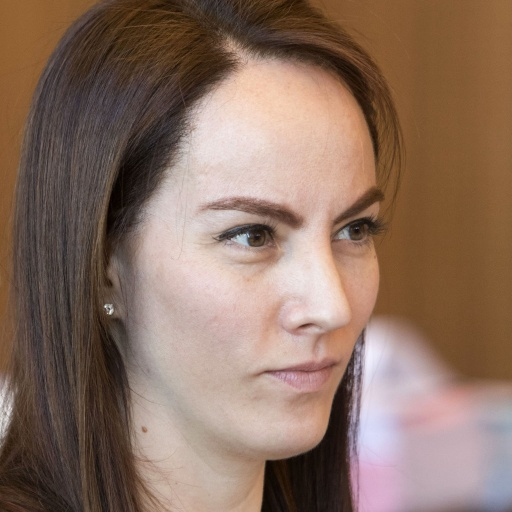
\includegraphics[width=4.35cm]{figures/diffrast_face/04114/target_hs}
    \caption{照片}
\end{subfigure}%
\begin{subfigure}{5.8cm}
\begin{tikzpicture}
    % 画一个表示透明的棋盘格
    \clip (0,0) rectangle (5.8cm,4.35cm);
    \begin{scope}[
        fgcolor/.style={fill=white!50!black},
        bgcolor/.style={fill=black!30!white},
        scale=0.1,
        ]
        \foreach \y in {0,1,...,43}{
            \foreach \x in {0,1,...,57}{
                \pgfmathparse{mod(\x+\y,2) ? "fgcolor" : "bgcolor"}
                \edef\rcolor{\pgfmathresult}
                \path[\rcolor] (\x ,\y) rectangle (1+\x,1+\y);
            }
        }
    \end{scope}
    \node [inner sep=0pt,outer sep=0pt,anchor=south west] at (0,0) {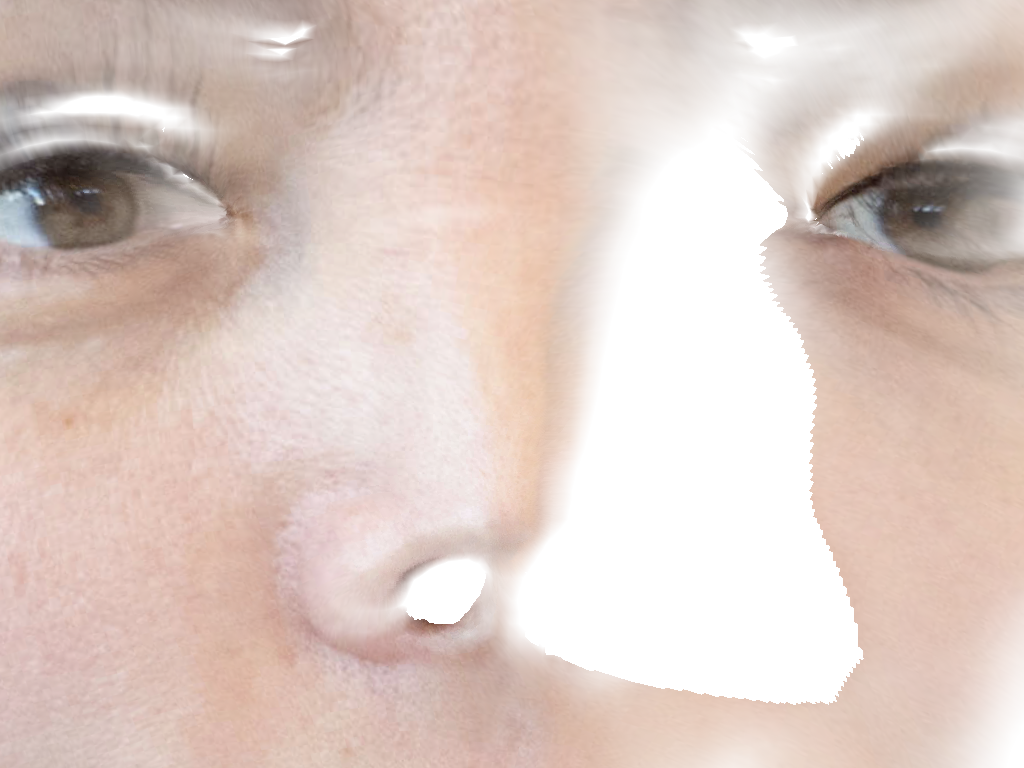
\includegraphics[width=5.8cm]{figures/diffrast_face/04114/uv_unwrap_full}};
\end{tikzpicture}%
\caption{纹理空间(局部)}
\end{subfigure}%
\begin{subfigure}{5.8cm}
\begin{tikzpicture}[blend mode=screen]
    \begin{scope}[transparency group]
        \begin{scope}[blend mode=multiply]
            \fill[blue] (0,0) rectangle (5.8cm,4.35cm);
            \node [inner sep=0pt,outer sep=0pt,anchor=south west] at (0,0) {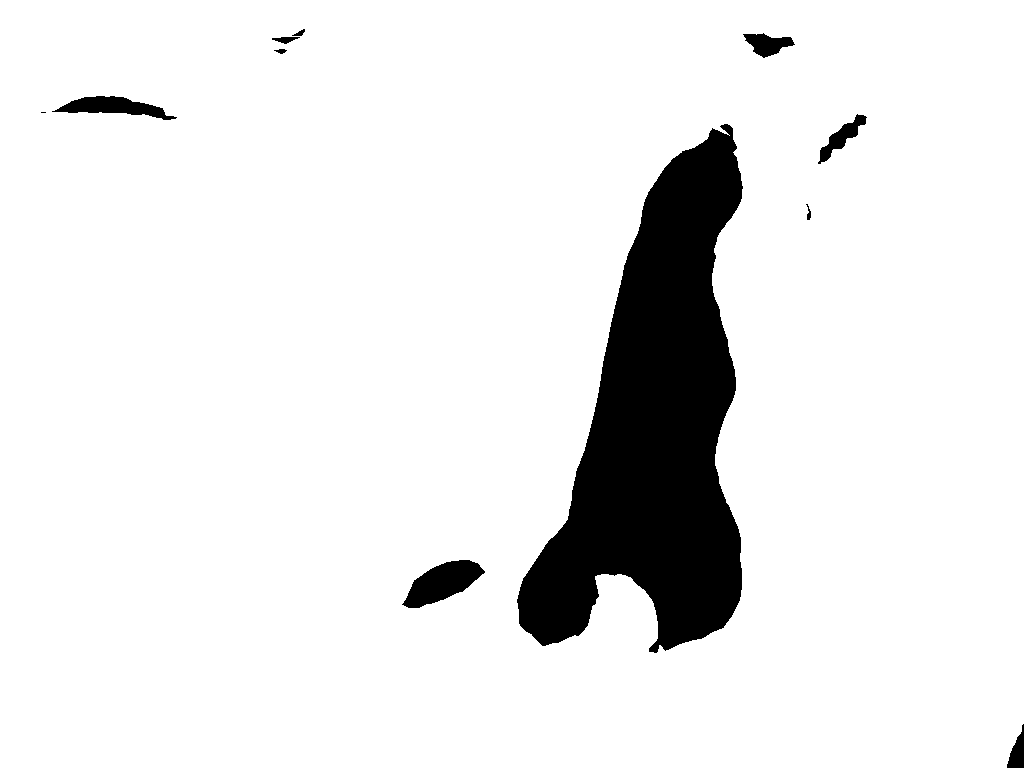
\includegraphics[width=5.8cm]{figures/diffrast_face/04114/uv_unwrap_normal}};
        \end{scope}
    \end{scope}
    \begin{scope}[transparency group]
        \begin{scope}[blend mode=multiply]
            \fill[green] (0,0) rectangle (5.8cm,4.35cm);
            \node [inner sep=0pt,outer sep=0pt,anchor=south west] at (0,0) {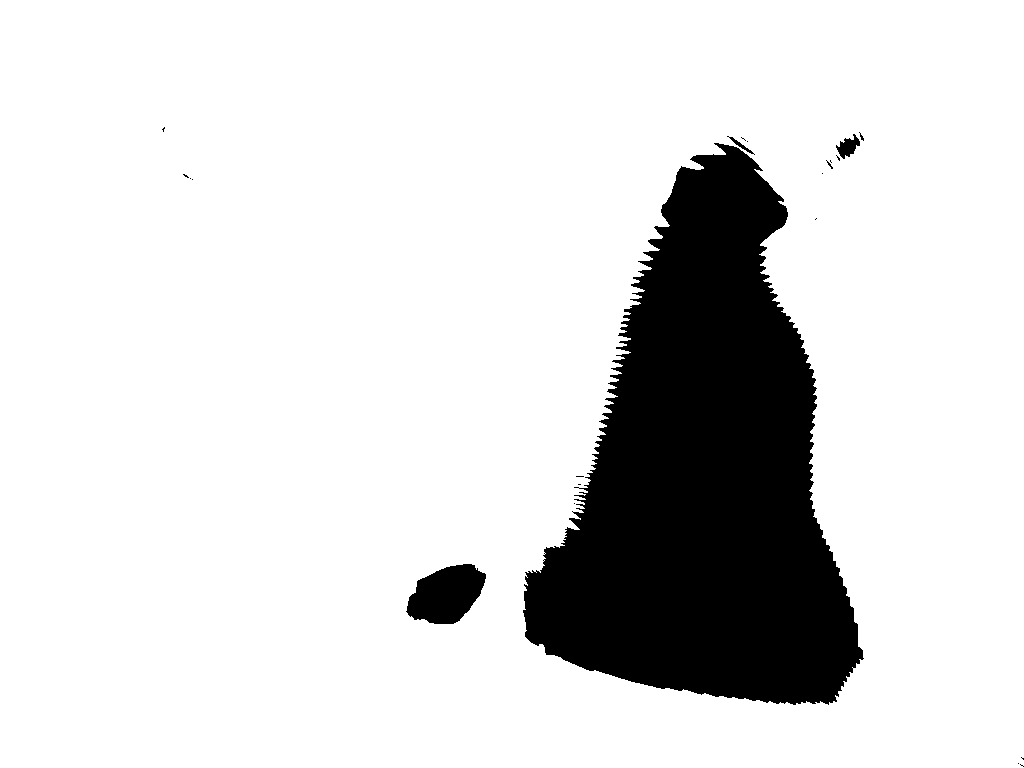
\includegraphics[width=5.8cm]{figures/diffrast_face/04114/uv_unwrap_occ}};
        \end{scope}
    \end{scope}
\end{tikzpicture}
\caption{有效区域判断策略}
\label{fig:unwrap_strategy}
\end{subfigure}
\caption[纹理迁移结果]{
    将照片(a)中的像素值迁移到纹理空间(b)中的结果。
    (b)中的透明度正比于法向与相机方向夹角的余弦值。
    (c)展示了两种策略的识别效果,
    其中蓝色区域表示法向与相机方向夹角小于90°的区域,
    绿色区域表示深度判断的未被遮挡区域,
    青色为两者的交集,即有效区域。
}
\label{fig:unwrap_result}
\end{figure}
如图\ref{fig:unwrap_result}展示了迁移的结果以及这两种策略的识别效果。
这两个策略各有优劣:
前者可准确识别有效和无效区域交界的位置;且法向与相机方向夹角越大其纹理分辨率越低,这也可以为后续补全的步骤提供依据,允许解算的纹理和补全的纹理间平滑过渡。
但该策略则无法区分朝向相机但被遮挡的部分。
后者则可以识别出被遮挡的区域,但由于数值计算的精度有限,需要设定阈值,因此无法准确判别交界的位置,图\ref{fig:unwrap_strategy}中可见交界处存在明显的锯齿,这是数值计算精度不足的体现。
本文选取两种策略识别的有效区域的交集作为最终的有效区域。

\paragraph{纹理补全}
由于本应用中以不同视角渲染的需求较低,本文仅使用了简单的策略对纹理中无效区域进行补全。
本文将3DMM预测的低频纹理与从照片中解算的纹理加权平均,其权重正比于法向与相机方向夹角的余弦:
\begin{equation}
\mathbf{\rho}_\mathrm{fused} = \begin{cases}
    \alpha \mathbf{\rho}_\mathrm{img} + (1-\alpha) \mathbf{\rho}, \alpha = \dfrac{\mathbf{v}\cdot\mathbf{n}}{\|\mathbf{v}\|} & \text{if像素位于有效区域} \\
\mathbf{\rho} & \text{otherwise}
\end{cases}
\label{eq:texture_fusion}
\end{equation}

最终,通过逆渲染的优化过程和照片到纹理空间信息迁移,即可获得所需的3D模型顶点坐标$\mathbf{S}$和其纹理$\mathbf{\rho}_\mathrm{fused}$。
该过程中得到的人脸姿态和环境光照信息也可以用于下游的渲染等任务中。

\section{实验结果}

本节将介绍本章方法的实验细节,以及其最终呈现的3D模型重新渲染的结果,并分析了其中各个环节的作用。

\paragraph{实验细节}
该实验的逆渲染过程使用PyTorch\citep{pytorch}和nvdiffrast实现。
长度单位为毫米。
本文使用Adam\citep{adam}优化器,光照参数、3DMM模型参数、平移量、旋转量、顶点偏移量的学习率分别为$10^{-3}$、$10^{-2}$、$10^{-2}$、$10^{-4}$、$10^{-3}$,其余参数为默认值。
可见性梯度扩展项的系数为$\alpha=10^{-7}$。
3DMM系数,顶点偏移、拉普拉斯、环境光照、光照修正场强度、梯度的正则项系数分别为
$10^{-5}$、$10^{-9}$、$40$、$10^{-4}$、$10^{-3}$、$10^{-3}$。
逆渲染的分辨率为$1024\times1024$,运行了1000次优化迭代。
在优化时,前100次迭代仅优化3DMM的反射率系数和SH光照参数,后续迭代则同时优化所有参数。
本实现在NVIDIA RTX3060显卡上,单张照片的逆渲染优化约需要16秒。
照片到纹理空间信息迁移使用OpenGL实现,仅需数毫秒。

\subsection{重新渲染效果}

\begin{figure}
\centering
    \begin{tikzpicture}[
        node distance=2pt and 0pt,
        image/.style={inner sep=0pt, outer sep=0pt},
    ]
        \node (a) [image] {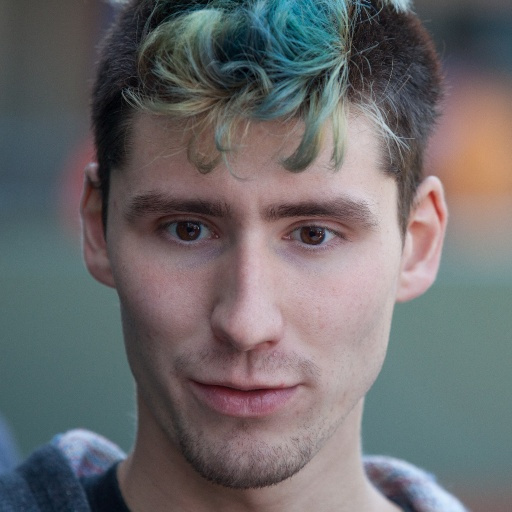
\includegraphics[height=1.27in]{figures/diffrast_face/00015/target_hs}};
        \node (b) [image,right=of a] {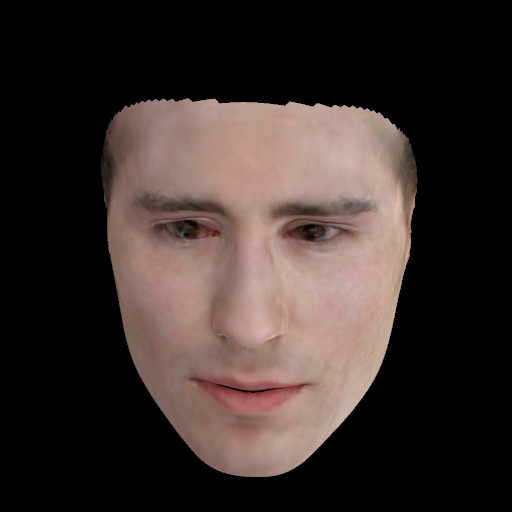
\includegraphics[height=1.27in,trim={2cm 0 2cm 0},clip]{figures/diffrast_face/00015/initial}};
        \node (c) [image,right=of b] {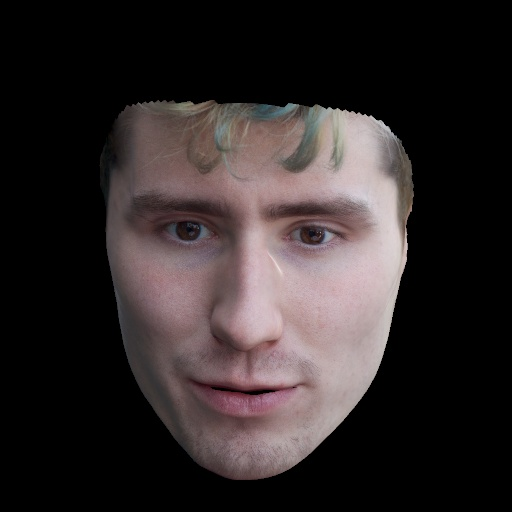
\includegraphics[height=1.27in,trim={2cm 0 2cm 0},clip]{figures/diffrast_face/00015/final_rerendered}};
        \node (d) [image,right=of c] {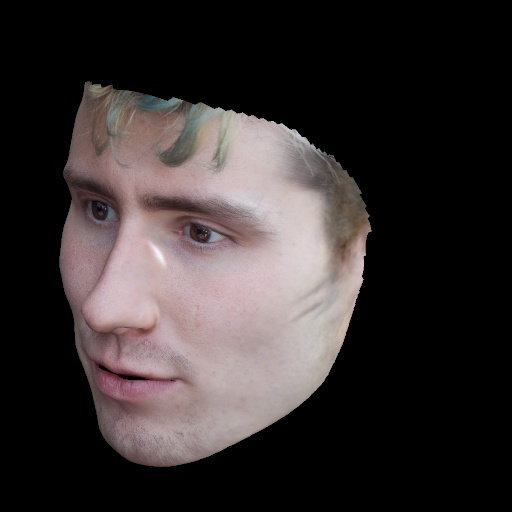
\includegraphics[height=1.27in,trim={1cm 0 3cm 0},clip]{figures/diffrast_face/00015/final_rot_rerendered}};
        \node (e) [image,right=of d] {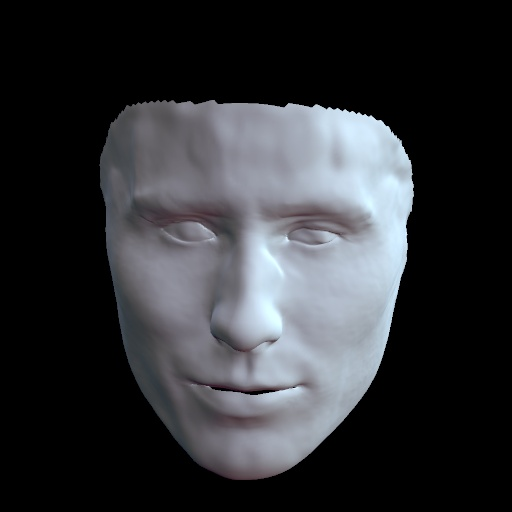
\includegraphics[height=1.27in,trim={2cm 0 2cm 0},clip]{figures/diffrast_face/00015/final_geo_rerendered}};
        \node (f) [image,right=of e] {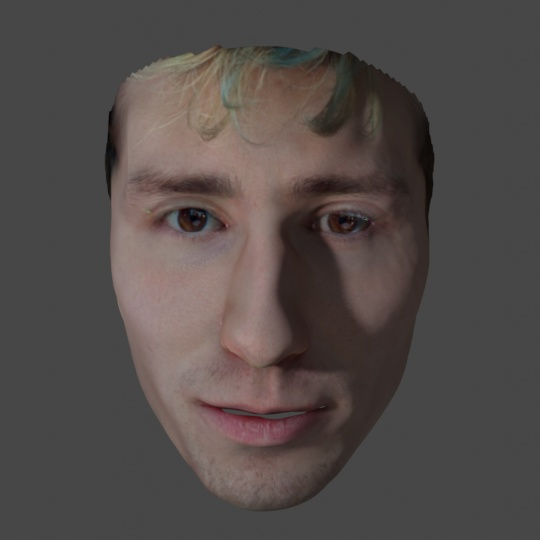
\includegraphics[height=1.27in,trim={2cm 0 2cm 0},clip]{figures/diffrast_face/00015/relight}};

        \node (a) [image,below=of a] {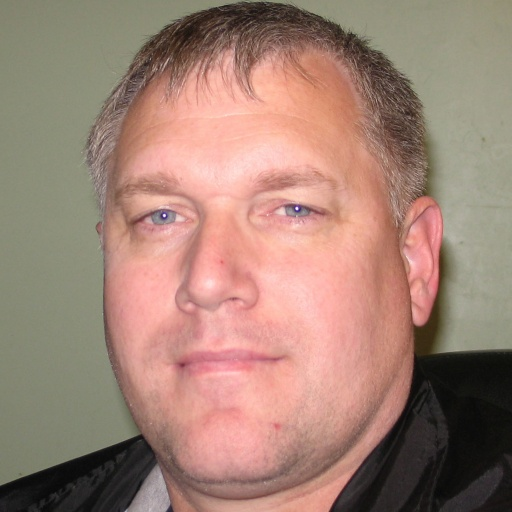
\includegraphics[height=1.27in]{figures/diffrast_face/00029/target_hs}};
        \node (b) [image,right=of a] {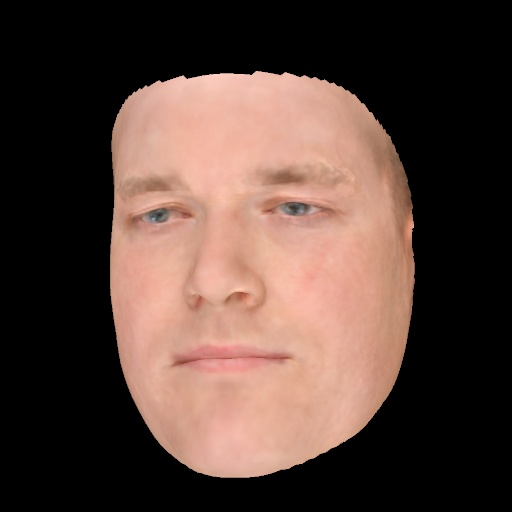
\includegraphics[height=1.27in,trim={2cm 0 2cm 0},clip]{figures/diffrast_face/00029/initial}};
        \node (c) [image,right=of b] {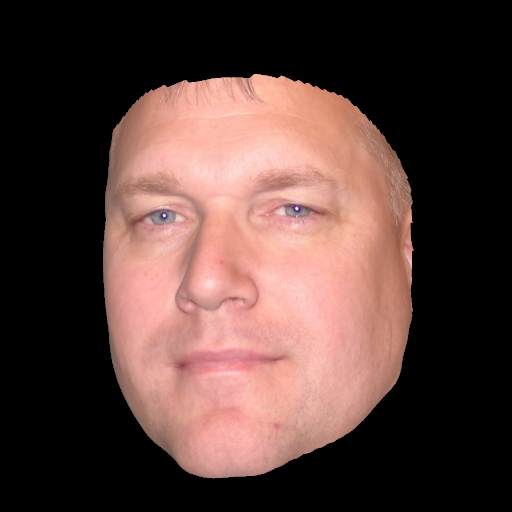
\includegraphics[height=1.27in,trim={2cm 0 2cm 0},clip]{figures/diffrast_face/00029/final_rerendered}};
        \node (d) [image,right=of c] {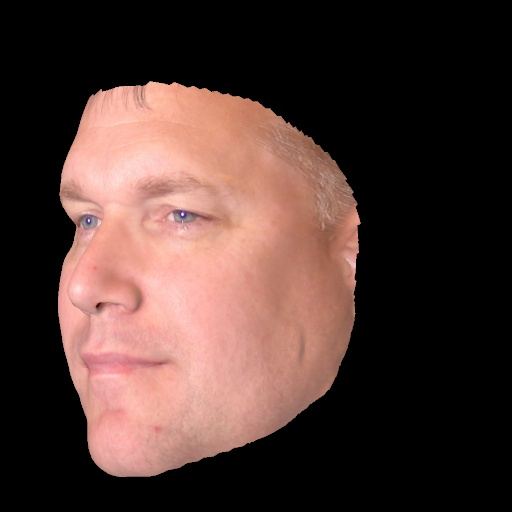
\includegraphics[height=1.27in,trim={1cm 0 3cm 0},clip]{figures/diffrast_face/00029/final_rot_rerendered}};
        \node (e) [image,right=of d] {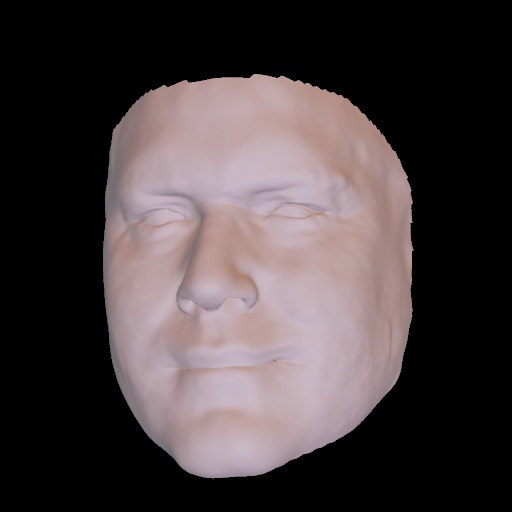
\includegraphics[height=1.27in,trim={2cm 0 2cm 0},clip]{figures/diffrast_face/00029/final_geo_rerendered}};
        \node (f) [image,right=of e] {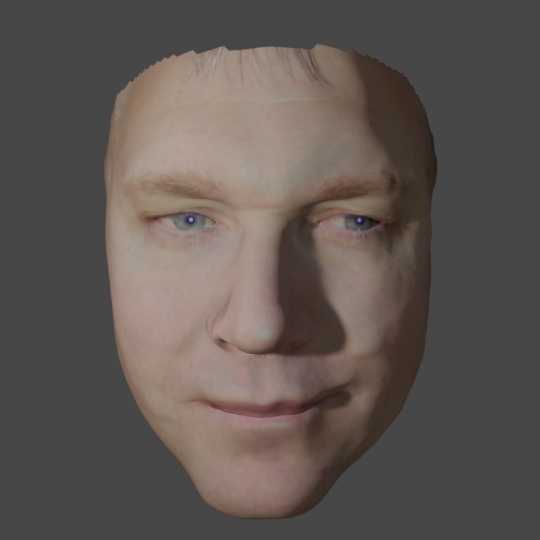
\includegraphics[height=1.27in,trim={2cm 0 2cm 0},clip]{figures/diffrast_face/00029/relight}};

        \node (a) [image,below=of a] {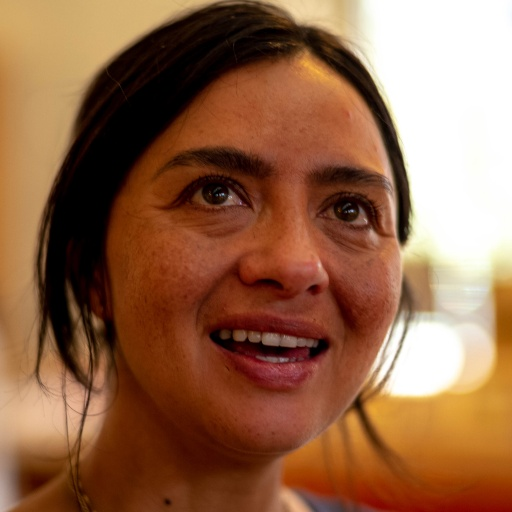
\includegraphics[height=1.27in]{figures/diffrast_face/00017/target_hs}};
        \node (b) [image,right=of a] {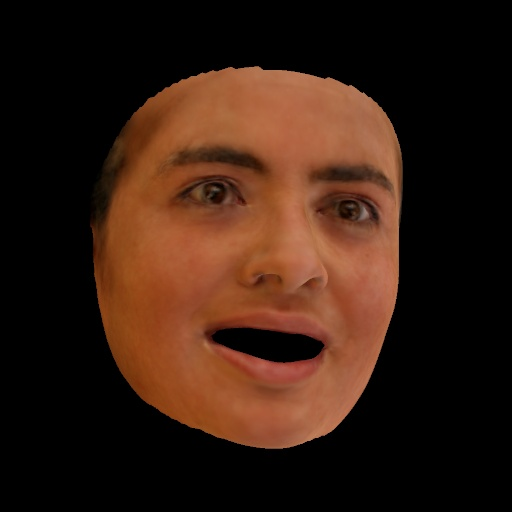
\includegraphics[height=1.27in,trim={2cm 0 2cm 0},clip]{figures/diffrast_face/00017/initial}};
        \node (c) [image,right=of b] {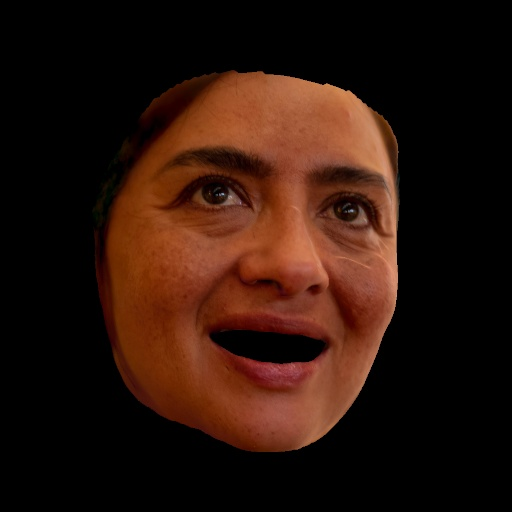
\includegraphics[height=1.27in,trim={2cm 0 2cm 0},clip]{figures/diffrast_face/00017/final_rerendered}};
        \node (d) [image,right=of c] {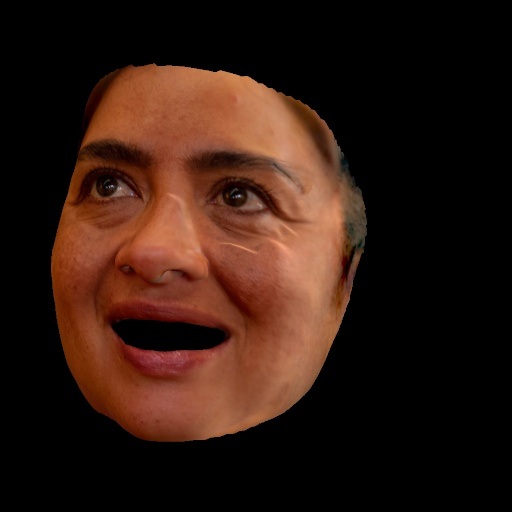
\includegraphics[height=1.27in,trim={1cm 0 3cm 0},clip]{figures/diffrast_face/00017/final_rot_rerendered}};
        \node (e) [image,right=of d] {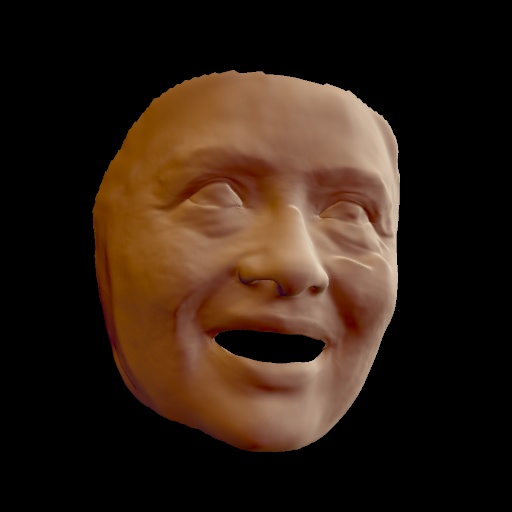
\includegraphics[height=1.27in,trim={2cm 0 2cm 0},clip]{figures/diffrast_face/00017/final_geo_rerendered}};
        \node (f) [image,right=of e] {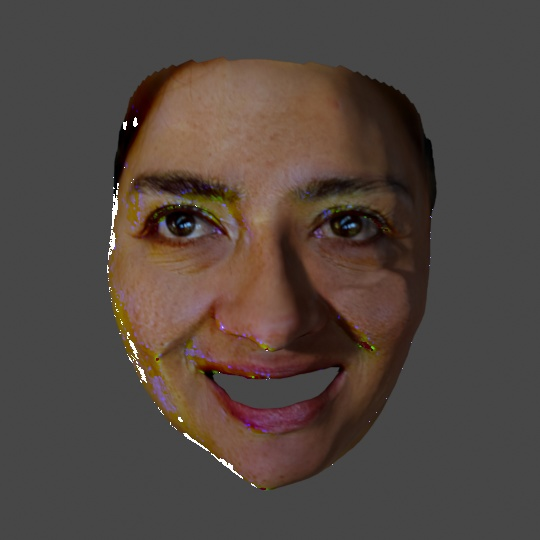
\includegraphics[height=1.27in,trim={2cm 0 2cm 0},clip]{figures/diffrast_face/00017/relight}};

        \node (a) [image,below=of a] {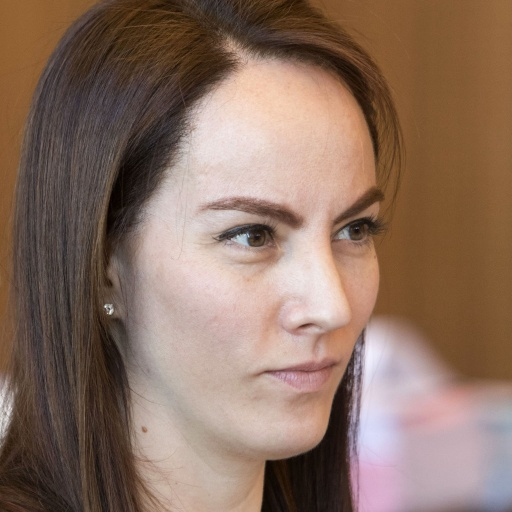
\includegraphics[height=1.27in]{figures/diffrast_face/04114/target_hs}};
        \node (b) [image,right=of a] {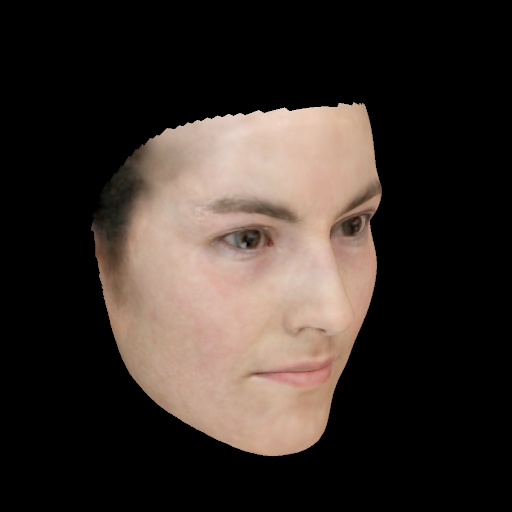
\includegraphics[height=1.27in,trim={2cm 0 2cm 0},clip]{figures/diffrast_face/04114/initial}};
        \node (c) [image,right=of b] {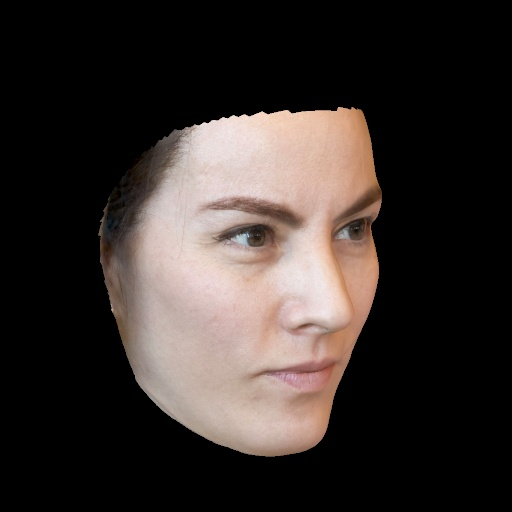
\includegraphics[height=1.27in,trim={2cm 0 2cm 0},clip]{figures/diffrast_face/04114/final_rerendered}};
        \node (d) [image,right=of c] {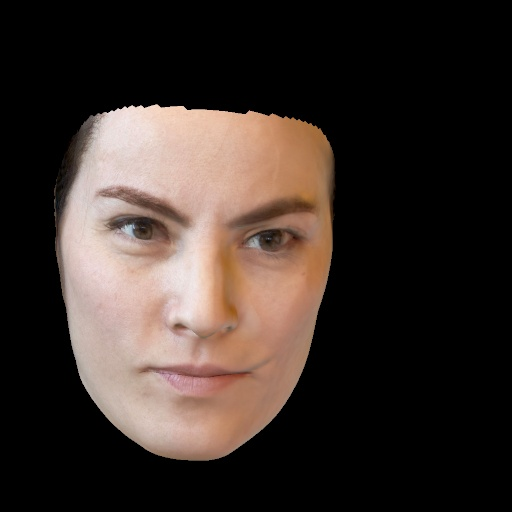
\includegraphics[height=1.27in,trim={1cm 0 3cm 0},clip]{figures/diffrast_face/04114/final_rot_rerendered}};
        \node (e) [image,right=of d] {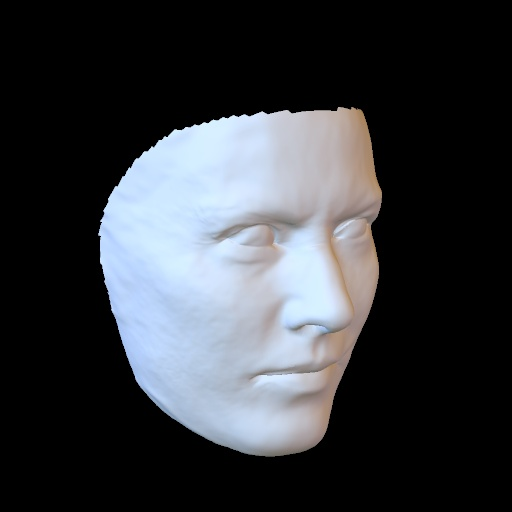
\includegraphics[height=1.27in,trim={2cm 0 2cm 0},clip]{figures/diffrast_face/04114/final_geo_rerendered}};
        \node (f) [image,right=of e] {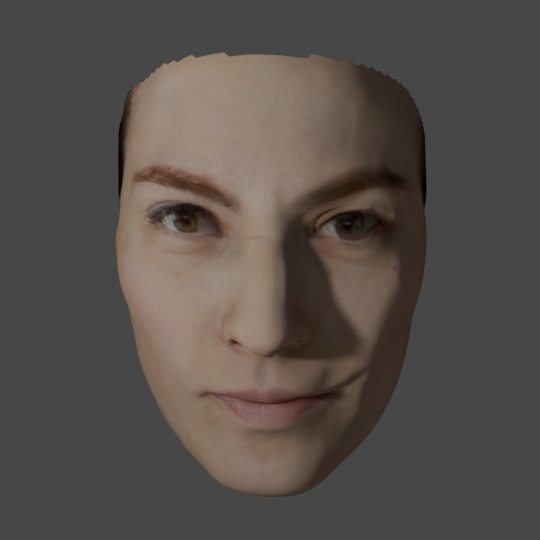
\includegraphics[height=1.27in,trim={2cm 0 2cm 0},clip]{figures/diffrast_face/04114/relight}};

        \node (a) [image,below=of a] {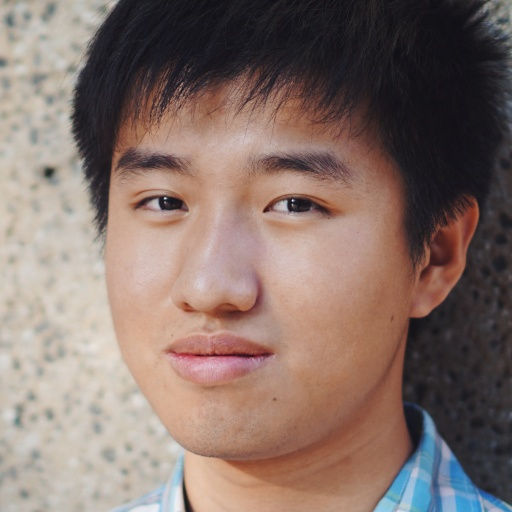
\includegraphics[height=1.27in]{figures/diffrast_face/04038/target_hs}};
        \node (b) [image,right=of a] {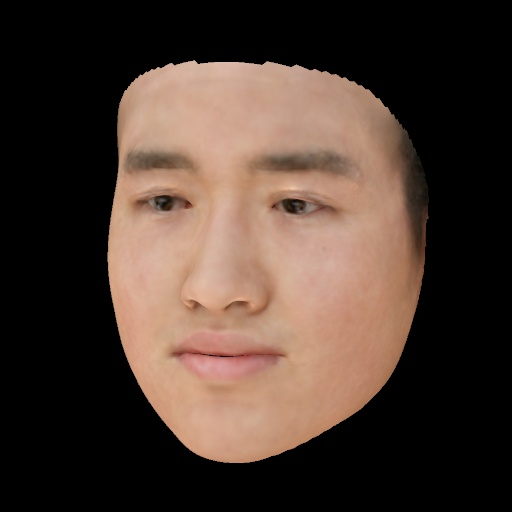
\includegraphics[height=1.27in,trim={2cm 0 2cm 0},clip]{figures/diffrast_face/04038/initial}};
        \node (c) [image,right=of b] {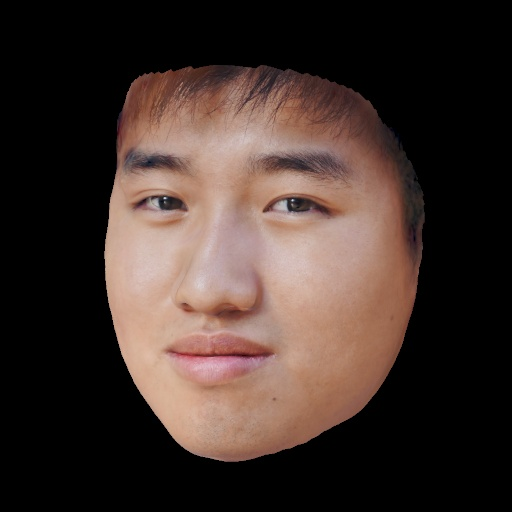
\includegraphics[height=1.27in,trim={2cm 0 2cm 0},clip]{figures/diffrast_face/04038/final_rerendered}};
        \node (d) [image,right=of c] {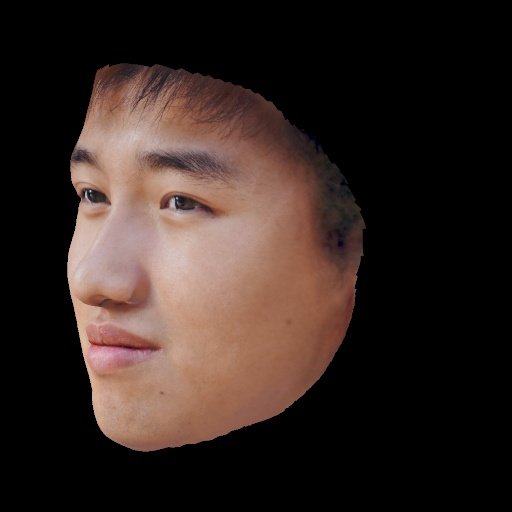
\includegraphics[height=1.27in,trim={1cm 0 3cm 0},clip]{figures/diffrast_face/04038/final_rot_rerendered}};
        \node (e) [image,right=of d] {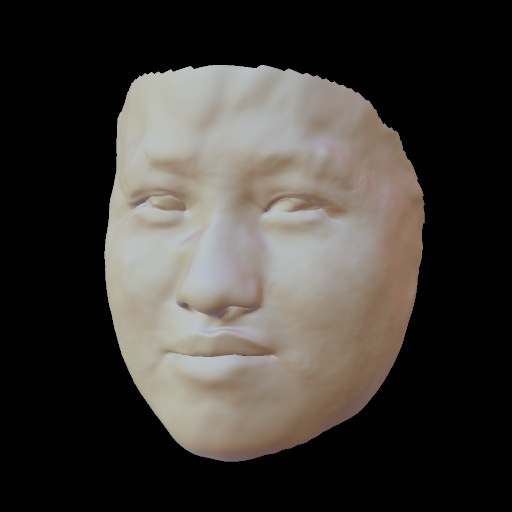
\includegraphics[height=1.27in,trim={2cm 0 2cm 0},clip]{figures/diffrast_face/04038/final_geo_rerendered}};
        \node (f) [image,right=of e] {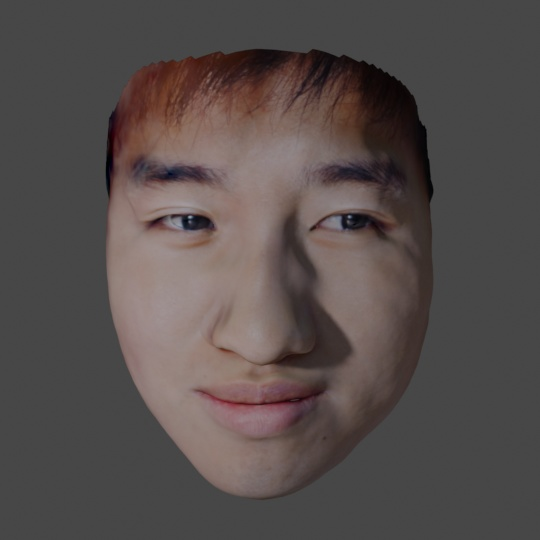
\includegraphics[height=1.27in,trim={2cm 0 2cm 0},clip]{figures/diffrast_face/04038/relight}};

        \small
        \node [below=of a] {(a)目标图像};
        \node [below=of b] {(b)初始化};
        \node [below=of c] {(c)重新渲染};
        \node [below=of d] {(d)新视角};
        \node [below=of e] {(e)几何\&光照};
        \node [below=of f] {(f)新光照};
\end{tikzpicture}
\caption[重建模型重新渲染的效果]{
    使用本文方法重建模型重新渲染的效果。
    (a)需要拟合的目标照片;
    (b)神经网络初始化的模型和光照;
    (c)使用本文方法重建的模型重新渲染的结果;
    (d)同一模型在旋转30°的新视角下重新渲染的结果;
    (e)逆渲染过程中估计的人脸几何和环境光照;
    (f)使用Blender在新的光照环境下重新渲染的结果。
    照片来自FFHQ数据集\citep{styleGAN}
}
\label{fig:rerender}
\end{figure}
本实现的目标是重建3D人脸模型并重新渲染输出较高质量的图像。
如图\ref{fig:rerender}展示了本文的实现重建的模型重新渲染的结果。
可以看到,本文的方法可以以很高的精度重新渲染获得以照片非常接近的结果。
同时,在新的视角和光照环境渲染也有不错的效果,良好地实现了既定目标。
与神经网络初始化的模型相比,本文的方法可以得到更准确的几何结构,以及显著更加丰富的纹理。

但是,作为一个传统优化算法,在巨大的解空间中,其鲁棒性并不如神经网络,特别是容易产生意外的小几何结构,例如在图\ref{fig:rerender}中的第一行中,鼻梁左侧出现了一个尖锐的突起,导致了明显的亮点。
这样的缺陷可以在未来结合更多有关人脸的先验知识得到改善。
作为权宜之计,也可以人工进行修复。

\begin{figure}
    \centering
    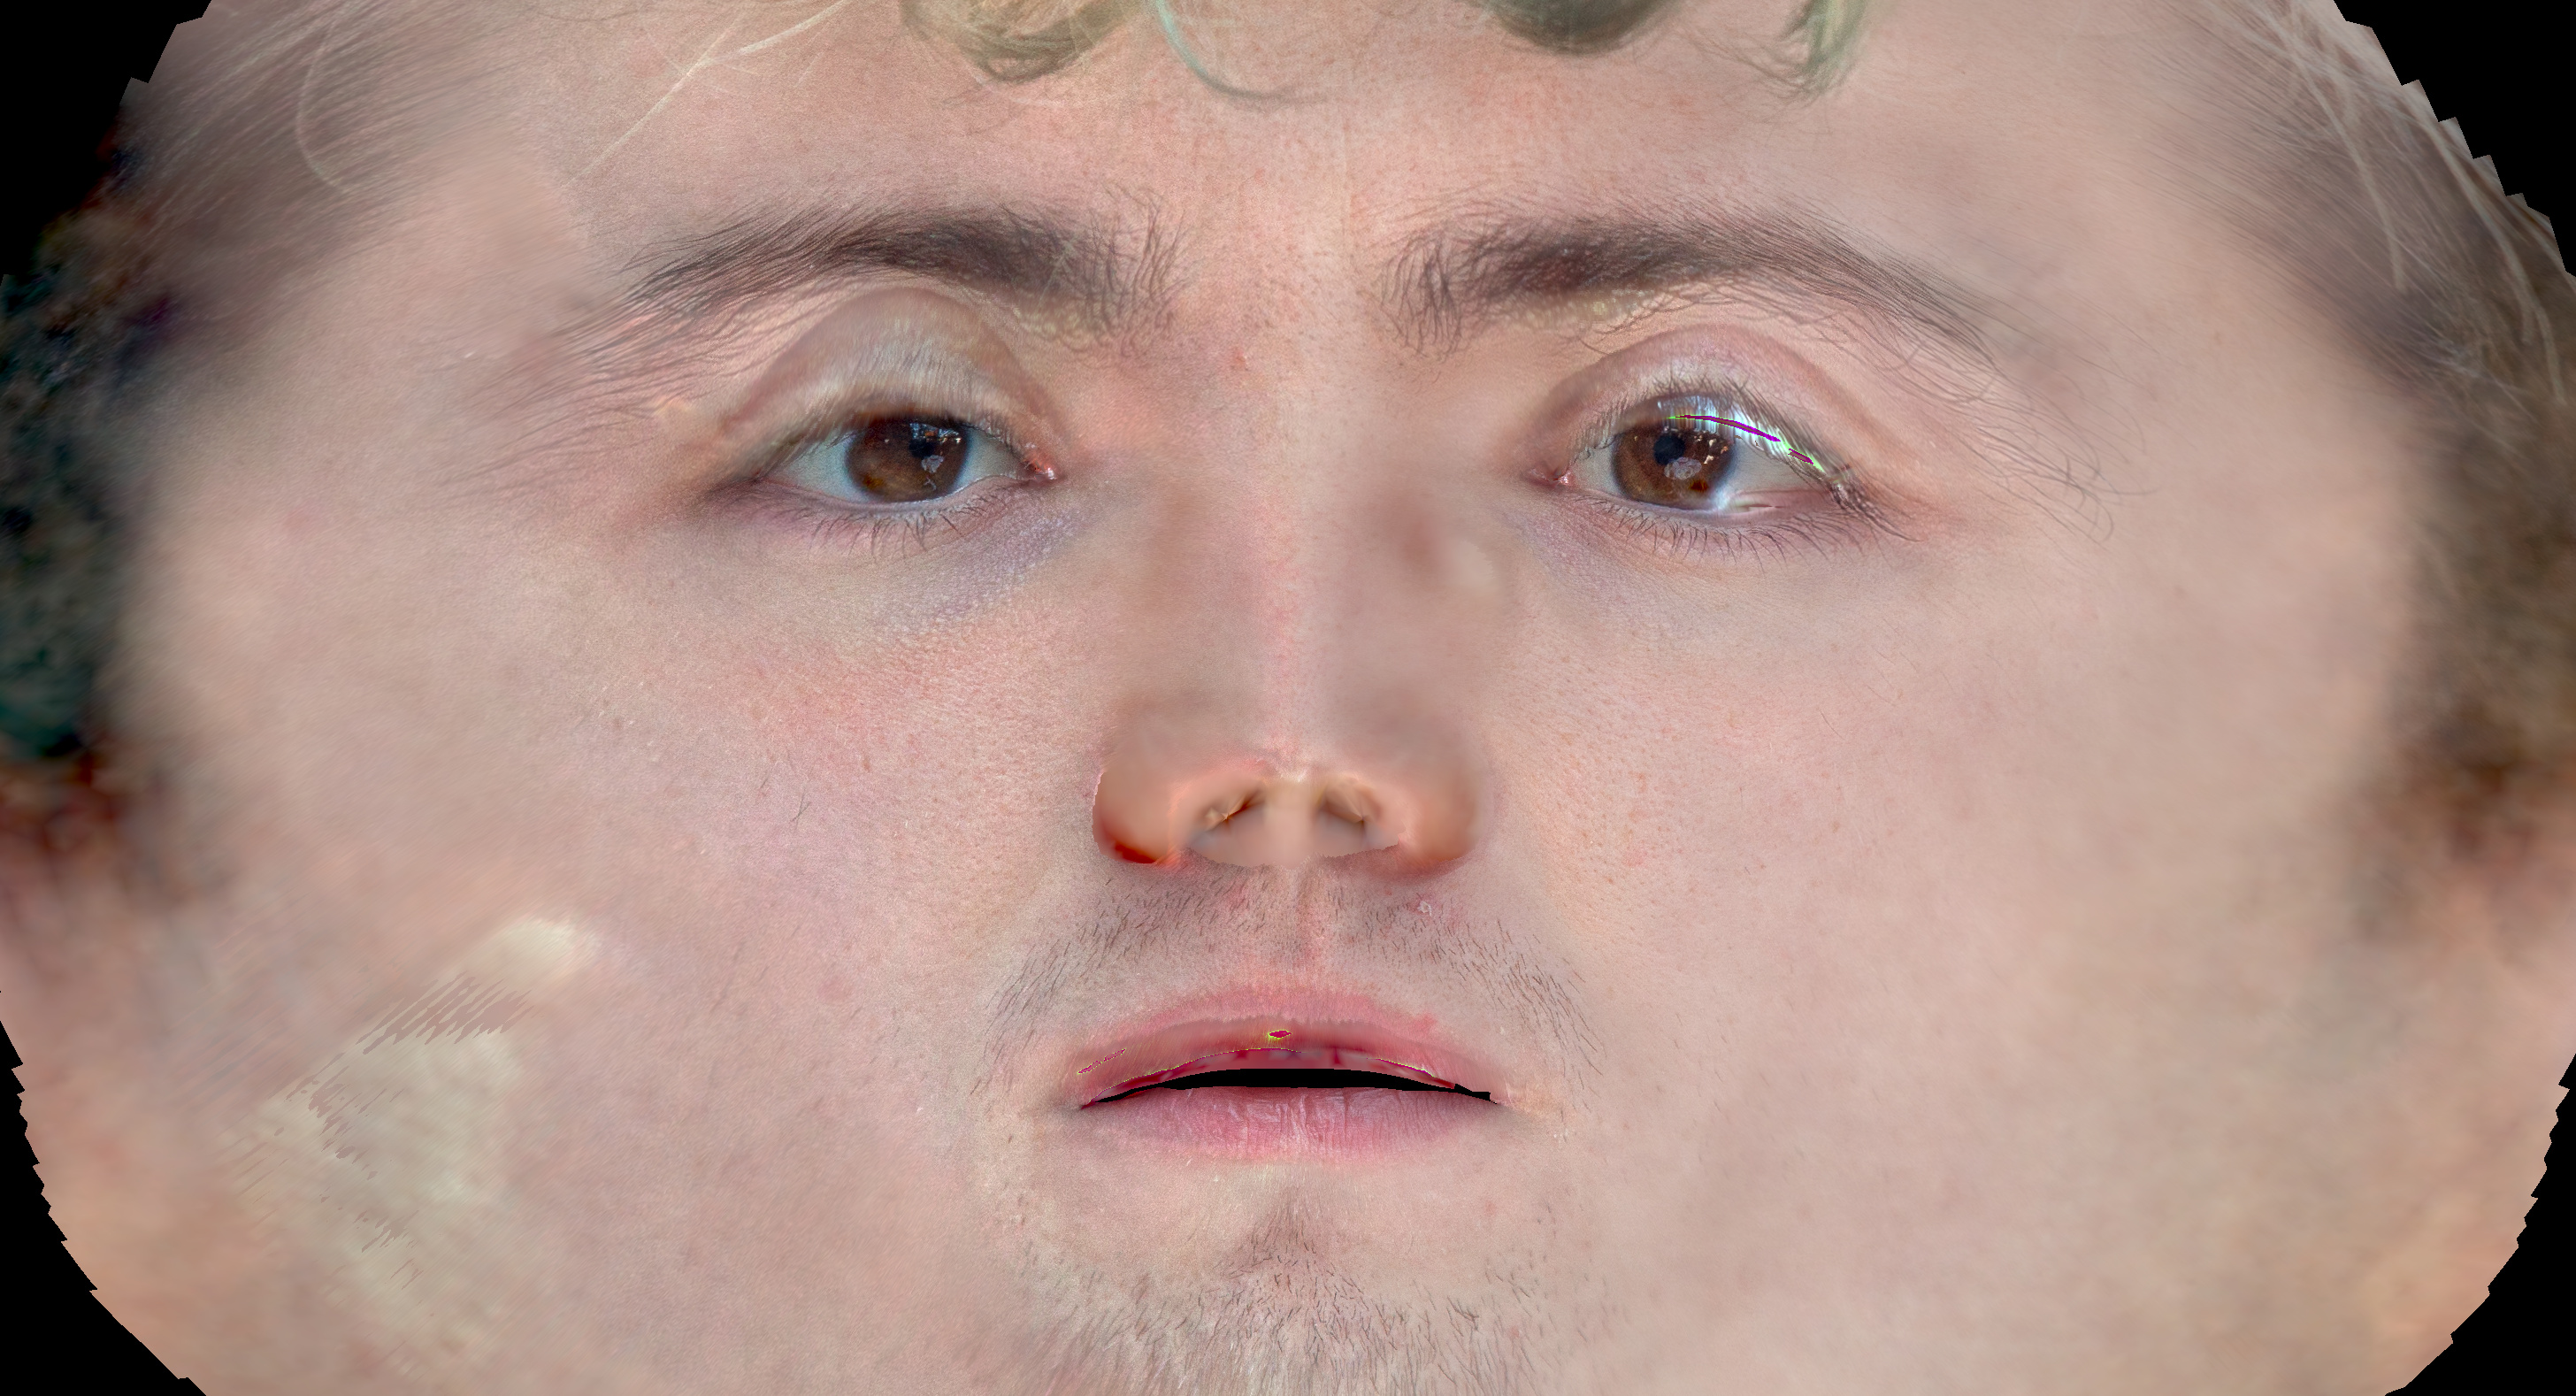
\includegraphics[width=\linewidth]{figures/diffrast_face/00015/final_diffuse}
    \caption{重建的反射率纹理贴图}
    \label{fig:diffuse_map}
\end{figure}
图\ref{fig:diffuse_map}展示了本文的实现重建的反射率纹理贴图。
该贴图对应了图\ref{fig:rerender}中的第一行。
可见,虽然照片中的人脸有明显的光照效果,纹理贴图中的颜色基本上是均匀的。
这说明本文实现的光照模型可较好地拟合并解耦照片中的光照效果。
同时,正脸部分毛孔和胡须的细节也被很好地保留了下来,两侧从照片中看不到的部分也被很好地补全了,且实现了平滑过渡。
这说明了本文使用的纹理补全方法的有效性。

\subsection{边缘对齐效果比较}
\label{sec:edge_align_exp}

\begin{figure}[tbh]
\centering
\begin{tikzpicture}[
    node distance=2pt and 0pt,
    image/.style={inner sep=0pt, outer sep=0pt},
    align result/.style={image, opacity=0.4}
]
    \node (target) [image] {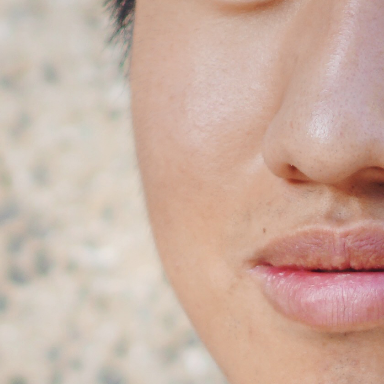
\includegraphics[height=1.55in]{figures/diffrast_face/04038/align_target}};

    \node (init) [image, right=of target] {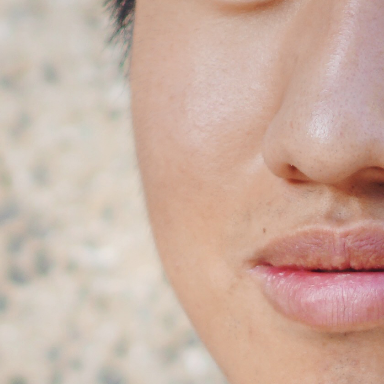
\includegraphics[height=1.55in]{figures/diffrast_face/04038/align_target}};
    \node [align result] at (init) {
\includegraphics[height=1.55in]{figures/diffrast_face/04038/alpha_init}};

    \node (landmark) [image, right=of init] {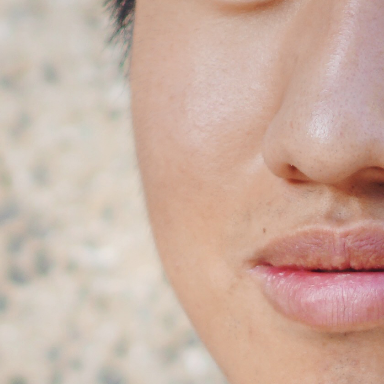
\includegraphics[height=1.55in]{figures/diffrast_face/04038/align_target}};
    \node [align result] at (landmark) {
\includegraphics[height=1.55in]{figures/diffrast_face/04038/alpha_landmark}};
    \node [image] at (landmark) {\input{build/figures/landmark.pgf}};

    \node (fitted) [image, right=of landmark] {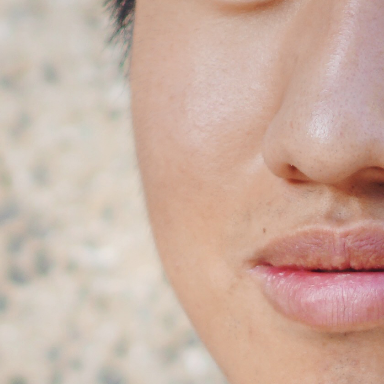
\includegraphics[height=1.55in]{figures/diffrast_face/04038/align_target}};
    \node [align result] at (fitted) {
\includegraphics[height=1.55in]{figures/diffrast_face/04038/alpha_fitted}};

    \small
    \node [below=of target] {(a)目标图像};
    \node [below=of init] {(b)神经网络预测};
    \node [below=of landmark] {(c)关键点约束};
    \node [below=of fitted] {(d)本文方法};
\end{tikzpicture}
\caption[人脸边缘对齐效果比较]{
    人脸边缘对齐效果比较。白色半透明覆盖层是人脸3D模型在图像上的投影。
    (c)中绿色圆点是2D检测方法的预测,红色是3D模型上标注的关键点在图像上的投影。
}
\label{fig:edge_alignment}
\end{figure}
本文的实现最大的特色是完全利用可微分渲染中的可见性梯度实现了模型与照片中边缘的对齐。
如图\ref{fig:edge_alignment}展示了本文的实现与其他方法的边缘对齐效果比较。
其中(b)是Deep3D\citep{deep3d}使用神经网络直接预测的方法,其训练过程使用了2D人脸关键点作为监督信号。
可能是由于其输入的分辨率较低,Deep3D的预测在高分辨率的图像中的对齐存在少量偏差。
由于本文方法需要针对每张图片迭代优化,因此为了公平比较,
图\ref{fig:edge_alignment}c展示了以类似Deep3D训练时使用的方法,针对单张图片以关键点作为监督信号进一步优化的结果。
可见虽然关键点已良好对齐,但这些监督信息仍不足以使模型和照片中的边缘精确对齐。
而本文的实现则能够很好地对齐边缘,且除了图片本身,不需要额外的监督信息。
这说明了第\ref{chap:method}章中提出的逆渲染方法的有效性。

需要指出,本文使用的适应未知背景的可微分渲染方法也可用于训练神经网络,从而实现类似Deep3D的实时效率。这方面还有待进一步研究。

\subsection{几何形状准确度定量比较}

\begin{table}
    \caption[FaceWarehouse数据集上的平均重建误差]{FaceWarehouse数据集上的平均重建误差(毫米)}
    \label{tab:facewarehouse}
    \centering
    \begin{tabular}{l|rrr}
        \toprule
        \multirow{2}{*}{方法} & \multicolumn{2}{c}{平均重建误差} & \multirow{2}{*}{运行时间} \\
        \cmidrule{2-3}
        & 小 & 大 \\
        \midrule
        Deep3D\citep{deep3d} & 1.81 & 1.91 & \textbf{2ms} \\
        \citet{GZCVVPT16} & \textbf{1.59} & 1.84 & 120s \\
        本文方法 & 1.66 & \textbf{1.81} & 20s \\
        \hspace{2ex} -无顶点偏移 & 1.70 & 1.90 & 20s \\
        \bottomrule
    \end{tabular}
\end{table}
为定量地评估本文的实现的几何形状准确度,本文在FaceWarehouse\citep{FaceWarehouse}数据集上进行了对比实验。
该数据集中包含了多个采集对象的多种表情的照片,以及其对应的3D模型。
仿照之前的方法,本文使用了FaceWarehouse数据集中地9个采集对象,各20种表情进行评估。
结果如表\ref{tab:facewarehouse}所示,
与之前的工作相同,本文分别在大小两种不同人脸裁剪区域下,展示了在共180个3D模型上的平均重建误差。
本文的实现在两种不同的人脸裁剪区域下的平均重建误差分别为1.66mm和1.81mm,均优于Deep3D的结果。
这说明本文提出的方法能有效利用照片中的信息,在已经非常准确的3D模型上进一步提高几何形状的准确度。
并能在仅使用了简单的像素损失的情况下与其他复杂的优化方法\citep{GZCVVPT16}相媲美。

此外,本文所优化的参数中包括额外的顶点偏移参数,这使重建的模型不完全受到3DMM低维空间的限制。
上文第\ref{sec:edge_align_exp}节中的实验已经说明现有方法不能很好地利用这些自由度。
而本文的方法能利用可见性梯度实现更稠密的监督信号,利用额外的自由度使模型能更好地对齐照片中的边缘,从而提升了几何形状的准确度。

\subsection{模型裁剪边缘的梯度处理效果}

\begin{figure}
    \centering
    \begin{subfigure}{1.6in}
        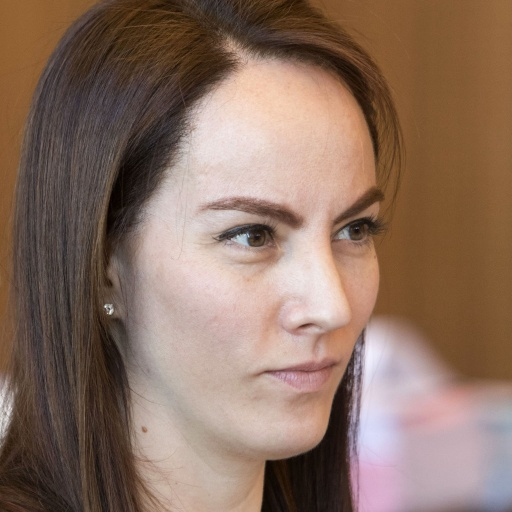
\includegraphics[height=1.6in]{figures/diffrast_face/04114/target_hs}%
        \caption{目标图像}
    \end{subfigure}%
    \begin{subfigure}{1.6in}
        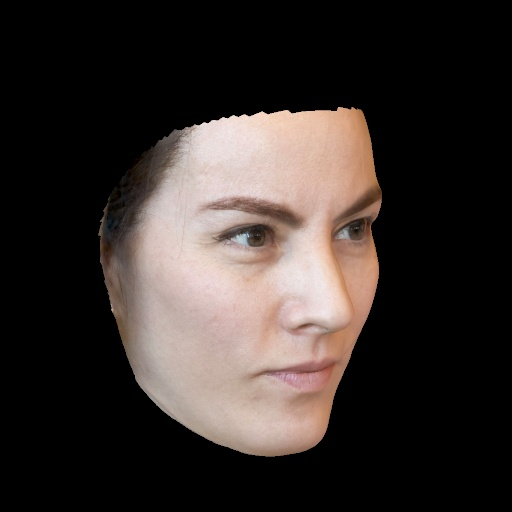
\includegraphics[height=1.6in]{figures/diffrast_face/04114/final_rerendered}%
        \caption{本文方法}
    \end{subfigure}%
    \begin{subfigure}{1.6in}
        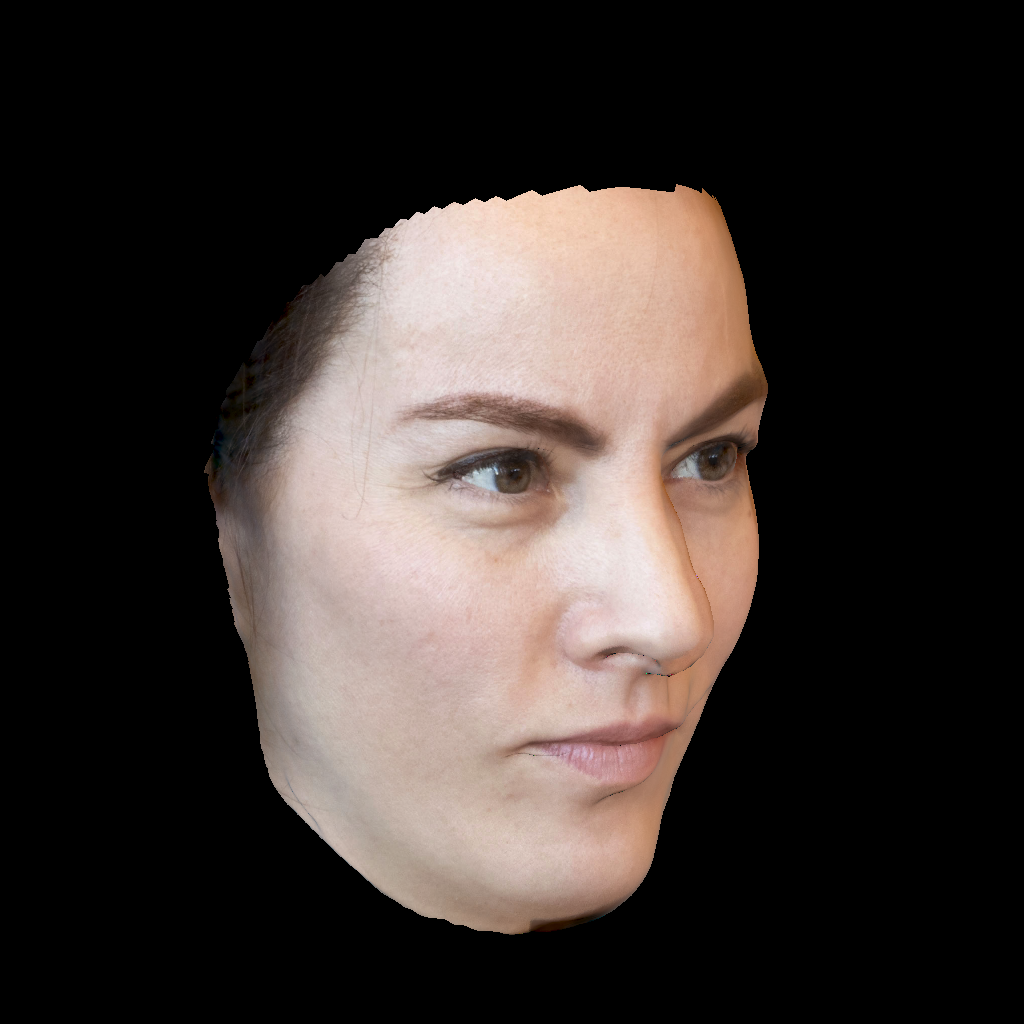
\includegraphics[height=1.6in]{figures/diffrast_face/04114/no_sdf}%
        \caption{不特殊处理}
        \label{fig:edge_gradient_no_sdf}
\end{subfigure}%
    \caption{基于SDF的裁剪边缘分类方法效果}
    \label{fig:edge_gradient}
\end{figure}
本文提出的可微分渲染方法应用在3D人脸重建时,会受到人脸模型人工裁剪的边缘的影响。
为验证本文提出的基于SDF的裁剪边缘分类方法的有效性,图\ref{fig:edge_gradient}展示了不同处理方法的效果比较。
对于原模型的下巴下方和额头上方的裁剪边缘,不做特殊处理时,可见性梯度试图指引这些边缘向外扩展以对齐到照片中的边缘。
然而照片中并不存在与之对应的边缘,这些边缘则将一直向外扩展,直到与其他正则化项达到平衡。
最终导致优化产生的网格与原模型的拓扑结构不一致,使得拟合质量劣化,且导致人脸模型重新拼接回完整的人体模型非常困难。
例如图\ref{fig:edge_gradient_no_sdf}中,算法将本应位于下巴处的网格用于拟合了照片中的脖子区域。
使用本文第\ref{sec:recon_sdf}节提出的方法即可过滤掉这部分产生于裁剪边缘的梯度,从而避免这种问题。

\section{局限性}

本章介绍的方法仅使用了少量建模在3DMM中的人脸先验知识,该信息中不包括人脸的几何和纹理细节。
而基于单张图片同时估计几何和纹理的问题是高度非适定的,因此本文也无法准确地重建这些细节。
目前,本文仅能重建较为低频的几何细节,此外未能表示的细节则全部会烘焙在反射率的纹理中。
本方法重建的几何形状也容易受到刘海,眼镜等遮挡物的影响,导致出现较大偏差。
这种方式虽然在原始视角和光照条件下渲染时可充分还原照片,但在大幅度改变视角或光照条件时,则会出现明显失真。
其中最明显的失真现象是新的光源产生的漫反射效果和烘焙在纹理中的镜面反射效果的不一致,它们两者将指示不同的光源方向。

此外,本文所使用的简单的朗伯特反射模型也过于简化,无法建模镜面反射导致的高光,以及人脸的次表面散射现象。
这同样会导致在改变视角或光照条件时,渲染出的结果出现失真。

\section*{本章小结}

在\hyperref[chap:method]{上一章}所提出的适应未知背景的逆渲染方法的基础上,本章将其成功应用于基于非受限环境照片的3D人脸重建中。
在将可见性梯度应用于人脸模型时,其裁剪边缘会产生异常梯度。
本章提出了一种基于SDF贴图的方法,能够有效地消除异常梯度,使人脸模型合理保持原有拓扑结构,提升了重建的实用性和准确性。
本章的实现还集成了现有神经网络回归方法为逆渲染提供初始化,并集成了一些传统方法生成高分辨率的纹理贴图,同时完成初步的光照效果解耦。
本章展示了该实现的最终重建效果,并通过实验验证了其中各个部分的有效性。
